\documentclass[a4paper,hidelinks,12pt]{report}

% Graphics and figures
\usepackage{graphicx}
\graphicspath{{images/}{./images/}{figures/}{./figures/}{./}}
\usepackage{float}

% Page layout
\usepackage{geometry}
\geometry{
 a4paper,
 left=30mm,
 top=25mm,
 bottom=20mm,
 right=20mm
}

\usepackage{multirow}
\usepackage{array}

% Algorithms
\usepackage{algorithm}
\usepackage{algorithmic}

% Mathematics
\usepackage{amsfonts}
\usepackage{amsmath}
\usepackage{mathtools}

% Text formatting and language
\usepackage[utf8]{inputenc}
\usepackage[english]{babel}
\usepackage{csquotes}

% Lists and enumerations
\usepackage{enumitem}

% Hyperlinks and references
\usepackage{hyperref}
\usepackage{xcolor}

% Appendices
\usepackage[toc,page]{appendix}

% Captions
\usepackage[labelfont=bf]{caption}

% Code listings
\usepackage{listings}
\usepackage{xcolor}

% Define colors for syntax highlighting
\definecolor{codegreen}{rgb}{0,0.6,0}
\definecolor{codegray}{rgb}{0.5,0.5,0.5}
\definecolor{codepurple}{rgb}{0.58,0,0.82}
\definecolor{backcolour}{rgb}{0.95,0.95,0.92}

% Configure listings style
\lstdefinestyle{solidity}{
    backgroundcolor=\color{backcolour},   
    commentstyle=\color{codegreen},
    keywordstyle=\color{blue},
    numberstyle=\tiny\color{codegray},
    stringstyle=\color{codepurple},
    basicstyle=\ttfamily\footnotesize,
    breakatwhitespace=false,         
    breaklines=true,                 
    captionpos=b,                    
    keepspaces=true,                 
    numbers=left,                    
    numbersep=5pt,                  
    showspaces=false,                
    showstringspaces=false,
    showtabs=false,                  
    tabsize=2,
    frame=single,
    rulecolor=\color{black}
}

\lstset{style=solidity}

% Tables
\usepackage{makecell}
% Add longtable only if you need tables spanning multiple pages
% \usepackage{longtable}

% Text decorations
\usepackage[normalem]{ulem}
\useunder{\uline}{\ul}{}

% Page orientation (only if needed)
% \usepackage{lscape}

% Set section numbering depth
\setcounter{secnumdepth}{5}

\begin{document}
\nocite{*}

% Front matter
\begin{titlepage}
    \begin{center}
        \vspace{1.0cm}
        
        \large
        VIETNAM NATIONAL UNIVERSITY OF HOCHIMINH CITY\\
        \large
        THE INTERNATIONAL UNIVERSITY\\
        \large
        SCHOOL OF COMPUTER SCIENCE AND ENGINEERING
        
        
        \vspace{3cm}
        \includegraphics[scale=0.8]{images/download.png}
        \vspace{3cm}
        
        \Huge
        \textbf{A Transparent and Granular Blockchain System for Verifiable Academic Provenance}\\

        \Large
        By\\
        {LE TIEN PHAT}
        \\
        {Student ID: ITITIU21273}
            
        \vspace{1.0cm}
        
            
        
            
        \large
        A thesis submitted to the School of Computer Science and Engineering \\
        in partial fulfillment of the requirements for the degree of \\
        Bachelor of Science in Computer Science
        
        \vfill
        Ho Chi Minh City, Vietnam\\
        2024
        
    \end{center}
\end{titlepage}
\begin{center}

\Large
\textbf{A Transparent and Granular
Blockchain System for Verifiable
Academic Provenance}


\vspace{3cm}

\large
APPROVED BY:\\


\underline{\hspace{5cm}},\\
Tran Thanh Tung, PhD\\
\vspace{1cm}


% \vspace{3cm}

THESIS COMMITTEE

\vspace{1cm}

\underline{\hspace{5cm}},\\
% Severus Snape, Professor\\
\vspace{1cm}

\underline{\hspace{5cm}},\\
% Uzumaki Naruto, Hokage\\
\vspace{1cm}

\underline{\hspace{5cm}},\\
% Roronoa Zoro, wait why is he here?\\
\vspace{1cm}

\underline{\hspace{5cm}},\\
% Yoda, Jedi Master\\
    
\end{center}







\pagebreak
\chapter*{Acknowledgement}
\addcontentsline{toc}{chapter}{Acknowledgement}

\begin{flushleft}
I want to express my sincere gratitude to Dr. Tran Thanh Tung. His dedicated guidance and support provided me with the optimal conditions to complete this thesis on "A Transparent and Granular Blockchain System for Verifiable Academic Provenance." Dr. Tran Thanh Tung generously shared invaluable professional knowledge and consistently inspired and motivated me throughout the learning and research process.

\vspace{0.5cm}

I also want to convey my sincerest thanks to all the professors and lecturers who taught and mentored me in my journey through the university. With their knowledge, experience, and commitment to the sector gave me the footing and confidence to achieve this project. I especially want to thank also Mr. Quang Dieu Nguyen and Mr. Duc Trung Luu, who took action as student mentors, for their references and wise thoughts that contribute strategies to this work.

\vspace{0.5cm}

Finally, I would like to express my deepest appreciation to my family and friends for their unwavering support throughout the development of my thesis. Their encouragement has been invaluable during this journey.
\end{flushleft}

\vspace{0.5cm}

\begin{flushright}
April, \\
Le Tien Phat.
\end{flushright}

% Table of contents
\tableofcontents{}

% Lists
\listoffigures
\addcontentsline{toc}{chapter}{List of Figures}
\listoftables
\addcontentsline{toc}{chapter}{List of Tables}

\pagebreak
\clearpage
\phantomsection
\addcontentsline{toc}{chapter}{List of Abbreviations}

\section*{List of Abbreviations}
\begin{description}
\item[API] — Application Programming Interface
\item[BCDiploma] — Blockchain Diploma
\item[CA] — Certificate Authority
\item[CLI] — Command Line Interface
\item[GDPR] — General Data Protection Regulation
\item[IPFS] — InterPlanetary File System
\item[JSON] — JavaScript Object Notation
\item[LRM] — Learning Record Management
\item[PKI] — Public Key Infrastructure
\item[PoS] — Proof of Stake
\item[PoW] — Proof of Work
\item[SIS] — Student Information Systems
\item[TPS] — Transactions Per Second
\item[ZKPs] — Zero-Knowledge Proofs
\end{description}

% Main content
\chapter*{Abstract}

\addcontentsline{toc}{chapter}{Abstract}
As education becomes increasingly modular and lifelong learning gains prominence, traditional credential verification systems remain limited to authenticating whole degrees or certificates. Current blockchain implementations reduce administrative burden but fail to capture the granular nature of learning achievements, creating opportunities for credential forgery through timeline manipulation and fabrication of learning histories. This research introduces IU-MiCert, a blockchain system that enhances existing credential management through verifiable academic micro-credential tracking with authentic timeline verification. Using advanced cryptographic data structures that improve storage and verification efficiency, IU-MiCert provides detailed learning record management while significantly strengthening protection against credential fraud through comprehensive timeline tracking. The system supplements existing credential verification by representing learning as a continuous, verifiable journey with cryptographically secured chronological records. This detailed academic history makes credential forgery substantially more difficult by creating comprehensive audit trails that expose inconsistencies in fabricated educational progressions. IU-MiCert enables students to build verifiable profiles incrementally, with each course, project, and achievement securely recorded with authentic timestamps within their broader educational context. For educational institutions, the system provides periodic update cycles that efficiently manage detailed learning records while minimizing blockchain storage costs. For business, especially employers, it enables verification of specific skills and authentic learning progression beyond single degree completion, supporting the increasingly important paradigm of skills-based hiring and lifelong learning verification. By enhancing traditional credential systems with detailed academic provenance, IU-MiCert transforms credential verification from basic authentication into comprehensive demonstration of authentic learning pathways, providing greater transparency, trust, and fraud protection for all stakeholders in the educational ecosystem.

\vspace{0.5cm}

\noindent\textbf{Keywords:} micro-credentials, academic provenance, blockchain verification, credential fraud prevention, learning timeline, verkle tree
\chapter{INTRODUCTION}
\label{ch:introduction}

\section{Motivation}
The educational landscape is transforming significantly as institutions move away from traditional degree-oriented models towards more flexible, modular learning pathways that extend beyond degree programs into that very life-long learning. The shifting landscape of our job markets recognizes a more idiosyncratic skill and competency value, as opposed to standard, more generalized assessments based on degree qualifications. Vietnam's national digital transformation strategy recognizes this shift, highlighting blockchain technology as a critical enabler for modernizing credential systems that can adapt to these emerging educational paradigms.

Traditional academic credentialing systems have severe constraints on describing and verifying the increasingly granular modes of learning. Traditional academic credentialing systems capture an entire degree or certificate with substantial verification, but they simply lack the capability to describe the rich mix of skills, projects, courses and competencies that represent a learner's actual educational journey. This gap creates a distinct divide between how learning occurs - incrementally, in diverse contexts, in multiple forms, and continuously throughout life - and how that learning receives formal recognition and verification.

The impact of this disconnect is significant. For students, their many learning accomplishments are distributed across different platforms and institutions disrupting a cohesive record of their learning progression and development of skills. For employers, the binary confirmation of degree completion doesn't provide insights into a candidate's specific knowledge and skills, creating unnecessary hurdles as employers seek to hire based on skills rather than labels. For educational institutions, the administrative burden of tracking and confirming credentials across institutional borders stifles student mobility and lifelong learning.

The recent blockchain implementations are addressing some of the issues around credential verification by increasing security and decreasing red tape. However, the majority of current solutions still treat whole credentials at the aggregate level instead of individual learning accomplishments. By treating degrees as an endpoint instead of a step along the continuing learning journey, we are stuck in a traditional model that serves neither modern employment nor education.

There are also technical limitations in relation to existing blockchain credentialing solutions that affect their viability and scale. As credentialing systems increase in scale because of increased detail in records, it becomes more complex in terms of storage and verification. Even though Merkle tree structures are secure, they can be inefficient when there are more micro-credentials to track. Even more impactful, the lack of standardized frameworks for tracking granular learning outcomes across learning institutions, there are issues with interoperability and opportunities for political forces to use timeline manipulation and fabrication to increase the potential for credential fraud.

The concept of academic provenance—the chronological record of a learner's educational achievements—emerges as a critical missing element in current systems. Without a transparent and verifiable timeline of credential acquisition, stakeholders cannot fully understand or trust the developmental progression that led to a learner's current competencies. In this context, the vulnerability of lack of historical verification could be the means by which credentialing fraud (e.g. backdating credential allotted to documenting achievement, and/or falsified educational paths with timelines of achievement) happens.

These interconnected challenges motivate the development of IU-MiCert, a blockchain system designed to enhance existing credential management through verifiable academic micro-credential provenance. By leveraging Verkle tree technology as an improvement over traditional Merkle trees, IU-MiCert provides more efficient storage and verification of detailed learning records while maintaining strong anti-forgery mechanisms through temporal verification. This approach serves as an upgrade to existing blockchain credential systems, adding granular tracking capabilities while preserving compatibility with traditional diploma verification.

Through IU-MiCert, we seek to enhance current credential verification systems by providing detailed academic provenance that makes credential forgery significantly more difficult, supporting the paradigm shift toward lifelong learning and skills-based assessment that characterizes modern educational landscapes.

\section{Problem Statement}
Current blockchain credential systems, while effective for whole degree verification, lack the capability to efficiently manage and verify the increasingly granular nature of modern education. This limitation creates opportunities for credential forgery and makes it difficult to establish authentic learning timelines. By implementing Verkle tree structures as an improvement over traditional Merkle trees, IU-MiCert addresses critical inefficiencies in academic credential management while significantly enhancing anti-forgery mechanisms through detailed provenance tracking.

Traditional credential systems and existing blockchain implementations focus primarily on validating complete degrees or certificates, creating a verification gap for the individual courses, projects, and skill-building experiences that comprise modern education. Without mechanisms to cryptographically verify the temporal sequence and authentic acquisition of micro-credentials, malicious actors can exploit this gap through timeline manipulation, backdating of achievements, and fabrication of learning progressions that are difficult to detect.

IU-MiCert implements an enhanced approach to credential verification that supplements existing systems with detailed micro-credential tracking. The system adds a comprehensive level of record-keeping for micro-credentials, which has provenance as an inextricable meaning of provenance. This system enables a comprehensive audit trail of learning achievements, with verifiable timestamps as part of a record of the overall educational ecosystem. This method crowds out fabricated credentials by exposing the timeline within the education records to see inconsistencies. This established provenance information provides additional layers of difficulty in proving forged credentials as well as affording stakeholders increased credibility in educational achievements. 

The use of Verkle trees over traditional Merkle trees provides improved efficiency in storing and verifying large numbers of micro-credentials, making this enhanced level of detail practically feasible for educational institutions to implement alongside their existing credential management systems, with a suitable costs.

\section{Scope}
The scope of this thesis is defined with the following key assumptions and infrastructure considerations to ensure the feasibility and applicability of the IU-MiCert system:

\vspace{0.3cm}

\textbf{1. Architectural Focus:} 
\begin{itemize}
Implementation of a Verkle tree-based architecture that provides improved efficiency over Merkle trees for storing and verifying micro-credentials as a supplement to existing credential management systems.
\end{itemize}

\textbf{2. Data Integrity and Authenticity:} 
\begin{itemize}
The credential data provided by the issuing institution is assumed to be accurate, complete, and from a verified source. This ensures that the system focuses on managing, issuing, and verifying credentials without addressing upstream validation processes.
\end{itemize}

\textbf{3. Infrastructure Assumptions:} 
\begin{itemize}
This thesis leverages existing infrastructure and cryptographic technologies, including:
\end{itemize}
\begin{itemize}
    \item A tamper-proof blockchain for storing commitment records, enabling decentralized trust without reliance on a single authority.
    \item Public Key Infrastructure (PKI) for managing and distributing public/private key pairs.
    \item Established cryptographic libraries for implementing the Verkle tree structure.
    \item Learning Management Systems and Student Information Systems that provide necessary data integration capabilities for seamless credential processing.
\end{itemize}

\textbf{4. Implementation Deliverables:}
\begin{itemize}
    \item A comprehensive system for deploying Verkle Trees of micro-credentials with term-based deployment cycles.
    \item Institutional commitment mechanisms that minimize on-chain storage requirements while maintaining detailed provenance.
    \item Intuitive user interfaces designed for students, employers, and educational institutions.
    \item Verification protocols that provide efficient proof generation and blockchain-powered validation regardless of system scale.
\end{itemize}

\textbf{5. User Environment:} 
\begin{itemize}
End-users and organizations adopting the system must have minimal technical requirements, such as internet access and standard computing devices, to interact with the interfaces provided.
\end{itemize}

\textbf{6. Performance Considerations:} 
\begin{itemize}
The infrastructure is designed to accommodate educational institution deployments, efficiently handling expected transaction volumes without significant performance degradation during peak verification periods.
\end{itemize}
By establishing these parameters, the thesis aims to design, implement, and demonstrate IU-MiCert as an enhancement to existing credential verification systems that provides detailed academic provenance while maintaining practical deployment feasibility.

\section{Objectives}
This thesis proposes designing, implementing, and evaluating IU-MiCert, a blockchain system that enhances existing credential management through verifiable academic micro-credential provenance. The project addresses the limitations of current systems that focus on complete degree verification while lacking detailed tracking capabilities that could prevent credential forgery. To summarize, the primary objectives of this thesis are as follows:

\vspace{0.3cm}

\textbf{1. Technical Contribution:}
\begin{itemize}
    \item Implement a Verkle tree-based architecture that improves upon traditional Merkle tree efficiency for managing large numbers of micro-credentials.
    \item Apply cryptographic mechanisms for establishing verifiable academic provenance with temporal verification capabilities.
    \item Design verification protocols that enhance anti-forgery protection through detailed timeline tracking.
\end{itemize}

\textbf{2. System Development:}
\begin{itemize}
    \item Design and implement smart contracts for micro-credential issuance and verification using Verkle tree structures with term-based deployment.
    \item Develop institutional commitment mechanisms that provide detailed provenance while minimizing on-chain storage requirements.
    \item Create comprehensive interfaces for students to manage receipts, employers to verify receipts, and an educational institutions system to issue and manage detailed learning records.
    \item Construct a full-stack solution that integrates with existing credential management systems to provide enhanced verification capabilities.
\end{itemize}

\textbf{3. Security and Performance Assessment:}
\begin{itemize}
    \item Conduct comprehensive evaluation of IU-MiCert's anti-forgery mechanisms, testing the system's ability to detect timeline manipulation and credential fabrication.
    \item Perform performance benchmarks comparing Verkle tree efficiency against traditional Merkle tree implementations for micro-credential management.
    \item Validate the system's practical feasibility for educational institution deployment alongside existing credential systems.
\end{itemize}

\textbf{4. Real-World Enhancement:}
\begin{itemize}
    \item Ensure that IU-MiCert's design can be practically integrated with existing blockchain credential systems as an enhancement rather than replacement.
    \item Develop integration guidelines for incorporating detailed micro-credential tracking into current learning management systems.
    \item Demonstrate IU-MiCert's effectiveness in improving credential authenticity verification while maintaining compatibility with traditional diploma verification processes.
\end{itemize}
\chapter{RELATED WORK}
\label{ch:related-work}

% TODO: Expand related work to 14 pages as per REPORT.md outline
% TODO: Include the following sections as outlined in REPORT.md:
% 1. Blockchain-based Credential Systems (partially covered)
% 2. Merkle Tree Approaches (partially covered)
% 3. Vector Commitment Schemes
% 4. Verkle Trees in Academia
% 5. Zero-Knowledge Proofs & Privacy
% 6. Research Gaps & Positioning

This chapter examines contemporary advancements in credential management systems, specifically focusing on decentralized and cryptographic methodologies that enhance security and operational efficiency. The review systematically identifies and analyzes the research gaps that these technological advancements have yet to address. The chapter establishes definitions of fundamental mathematical concepts that underpin current systems, providing essential context for understanding both the capabilities and limitations of existing credential management approaches. These foundational elements are critical for establishing the theoretical framework that supports the development of the IU-MiCert protocol and positioning it within the broader landscape of academic credential verification systems.

\section{Current Advancements}
This section reviews the evolutionary progression of decentralized credential management systems, tracing the technological advancement from foundational blockchain implementations to sophisticated cryptographic commitment schemes that enable scalable and privacy-preserving credential verification.

\subsection{Foundational Blockchain Implementations}

The earliest blockchain-based credential systems established the fundamental principles of decentralized verification while revealing critical limitations in scalability and granularity. The MIT Media Lab's BlockCerts \cite{blockcerts_mit} established foundational approaches by storing credential hashes on Bitcoin blockchain, enabling decentralized verification without central authority dependence. This pioneering system demonstrated the viability of blockchain-based credential integrity but treated credentials as monolithic entities, lacking support for the micro-credential granularity that modern educational paradigms require.

Building upon these foundations, Ethereum-based systems introduced smart contract automation for credential management. Nguyen et al.'s Certificate Verifying Support System (CVSS) \cite{nguyen2018cvss} advances blockchain-based credential management through smart contract automation and Know-Your-Customer principles. While CVSS demonstrates practical implementation in educational settings, it faces substantial scalability limitations due to requiring individual smart contracts per student, creating prohibitive costs for large-scale deployment.

Educational-specific blockchain platforms further refined these approaches for institutional environments. Turkanović et al.'s EduCTX platform \cite{turkanovic_eductx} enables credit transfer through consortium blockchain architecture, supporting educational mobility through credit accumulation validation. Similarly, Hyperledger Fabric-based implementations \cite{khan_hyperledger} have gained traction due to permissioned network characteristics suitable for institutional environments, with frameworks demonstrating smart contract-based credential validation with IPFS storage integration.

\subsection{Merkle Tree Approaches}

The integration of Merkle tree structures marked a significant advancement in cryptographic verification for credential systems, enabling efficient membership proofs and tamper detection. Le et al.'s IU-TransCert system \cite{le_iutranscert} demonstrates practical implementation of Auditable Merkle Tree structures for academic certificate issuance, confirmation, and auditing, providing features for credential revocation and selective information dissemination. Rasool et al.'s Docschain \cite{rasool_docschain} further advances Merkle tree applications by enabling blockchain-based verification of physical transcripts through IoT camera integration, though computational expenses arise from OCR processing requirements.

However, traditional Merkle tree implementations in educational contexts, while foundational, presented notable drawbacks. A primary concern became the substantial proof sizes required for verification. As the number of credentials grew, so did the accompanying proofs, which consist of all sibling hashes along the path to the root. This logarithmic scaling (O(logN)) still led to considerable data overhead, impacting efficiency. Furthermore, the necessity of disclosing a complete path for verification raised privacy issues regarding the relationships between credentials. Coupled with this, the computational demands and storage implications of tree rebalancing due to credential additions or revocations also scaled unfavorably with institutional expansion, hindering dynamic credential management.

Multi-signature authentication mechanisms built upon Merkle tree foundations attempted to address trust distribution in credential issuance processes. Wolfgang et al. \cite{wolfgang} demonstrate improved security through distributed authority control, though their approach lacks integration with temporal verification systems necessary for establishing authentic learning progression timelines.

% TODO: Add remaining sections to meet 14-page requirement as per REPORT.md:
% - Vector Commitment Schemes
% - Verkle Trees in Academia
% - Zero-Knowledge Proofs & Privacy
% - Research Gaps & Positioning

% TODO: Specifically address the use of Ethereum's go-verkle library in the implementation
% TODO: Compare with alternative approaches like zk-SNARKs for privacy preservation
% TODO: Discuss efficiency differences between Merkle and Verkle trees in academic credential contexts

\subsection{Vector Commitment Approaches}

Vector commitment schemes emerged as a sophisticated solution to the scalability and privacy limitations inherent in traditional tree-based approaches. These advanced cryptographic primitives enable constant-sized commitments to vectors of arbitrary length, providing efficient membership proofs without revealing vector structure or requiring path disclosure.

Nguyen and Tran's IU-VecCert \cite{nguyen2024iuvec} protocol represents significant progress in addressing scalability challenges through non-interactive vector commitment schemes that enable efficient credential issuance and verification. The IU-VecCert approach provides constant-sized proofs for credential verification regardless of the total number of issued credentials, representing a substantial improvement over traditional commitment schemes that suffer from linear proof size growth.

Advanced cryptographic accumulators built upon vector commitment principles have demonstrated potential for managing large-scale credential databases while maintaining efficient verification properties. Research has proposed dynamic bilinear-map accumulators that enable constant-sized proofs and efficient revocation mechanisms, showing promise for scalable credential management while requiring integration with hierarchical structures necessary for representing complex relationships between individual micro-credentials and composite qualifications.

\subsection{Verkle Tree Integration}

Verkle tree structures represent the current state-of-the-art advancement in cryptographic commitment schemes for educational applications, combining the hierarchical organization benefits of traditional Merkle trees with the constant-sized proof advantages of vector commitments. These structures enable efficient membership proofs with constant-sized verification regardless of tree size, addressing fundamental scalability limitations while maintaining the organizational benefits of tree-based structures.

The integration of Verkle trees with polynomial commitment schemes enables sophisticated selective disclosure mechanisms that preserve privacy while supporting granular credential verification. Unlike traditional Merkle trees that require complete path disclosure, Verkle trees enable selective revelation of credential subsets without exposing the broader credential structure or relationships.

However, existing educational blockchain systems have not yet leveraged Verkle trees for establishing verifiable academic provenance or supporting granular micro-credential management. Current implementations focus primarily on the technical cryptographic properties rather than developing comprehensive frameworks for tracking temporal relationships between micro-credentials and their aggregation into broader qualifications.

\subsection{Contemporary Cryptographic Integration}

Zero-knowledge proofs are increasingly complementing advanced commitment schemes to boost privacy. For instance, Delgado-von-Eitzen et al. \cite{delgado_gdpr} suggest GDPR-compliant frameworks for selective academic record disclosure, preserving privacy while ensuring verification integrity through sophisticated cryptography. While alternative hash-based verification systems reduce storage by comparing document hashes with blockchain references, they crucially fail to capture temporal relationships between credentials. This omission hinders the detection of fraudulent sequences and the establishment of legitimate educational progression. The convergence of these cryptographic methods offers pathways to comprehensive credential management systems addressing scalability, privacy, and provenance in modern education. However, a significant gap remains in unifying these technologies into frameworks that support granular micro-credential tracking with verifiable temporal provenance.

\section{Research Gaps}
Based on the comprehensive literature review, several critical research gaps emerge that hinder the practical deployment of scalable credential verification frameworks.
A primary gap exists in the continued reliance on traditional Merkle tree structures. Despite implementations like IU-TransCert \cite{le_iutranscert} and BlockCerts \cite{blockcerts_mit}, Merkle trees suffer from logarithmic proof sizes that create substantial storage overhead. Systems like CVSS \cite{nguyen2018cvss} exemplify this limitation where "using one smart contract per student results in significant financial and environmental costs per diploma."
Current systems also exhibit inadequate privacy preservation mechanisms. While frameworks attempt GDPR compliance \cite{delgado_gdpr}, they lack cryptographic sophistication for efficient privacy-preserving verification, typically requiring complete credential exposure during verification processes.
A significant gap exists in the underutilization of advanced cryptographic commitment schemes, particularly Verkle trees. Current systems like EduCTX \cite{turkanovic_eductx} and recent implementations like IU-VecCert \cite{nguyen2024iuvec} demonstrate progress but fail to address fundamental scalability limitations through advanced tree structures that provide constant-size proofs.
Additionally, existing solutions lack integrated support for complex educational hierarchies. Systems treat credentials as isolated entities, failing to capture relationships between micro-credentials, course components, and composite academic qualifications. This limitation prevents comprehensive verification of complete academic journeys, where individual micro-credentials should collectively prove mastery of broader educational objectives and degree requirements.
The IU-MiCert system addresses these gaps by leveraging Verkle tree architectures to achieve constant-size proof generation while implementing smart aggregation of proofs that enables provable academic journey reconstruction through interconnected micro-credential verification, bridging theoretical cryptographic advances with practical educational blockchain deployment.


\section{Theoretical Background}
This section establishes the foundational concepts necessary for understanding the proposed IU-MiCert protocol, covering educational micro-credential systems, blockchain technology, and the advanced cryptographic primitives that enable scalable credential verification.

\subsection{Micro-Credentials in Educational Systems}
\label{subsec:microcredentials}

Micro-credentials represent a fundamental shift in educational credentialing, providing granular recognition of specific skills and competencies. As defined by Chukowry et al. \cite{chukowry2021future}, a micro-credential is "a program that helps students to build skills outside the classroom by providing courses that cover specified skills," typically spanning 10 weeks to one year in duration.

Unlike traditional degree programs, micro-credentials offer several key characteristics:
\begin{itemize}
   \item \textbf{Granularity}: Recognition of specific competencies rather than broad academic achievements
   \item \textbf{Modularity}: Can be combined to form larger qualification frameworks
   \item \textbf{Immediacy}: Shorter duration enables rapid skill acquisition and verification
   \item \textbf{Industry Alignment}: Direct correlation with market-demanded skills
\end{itemize}


The hierarchical nature of educational systems creates natural relationships between micro-credentials, where individual achievements contribute to broader learning outcomes. This hierarchical structure forms the foundation for the tree-based organization employed in IU-MiCert.

\subsection{Blockchain Technology}
\label{subsec:blockchain_technology}

Blockchain technology emerged with Bitcoin as the foundational innovation that enabled decentralized digital currency without trusted intermediaries \cite{nakamoto2008bitcoin}. Nakamoto's seminal work introduced the concept of a "distributed ledger that maintains a continuously growing list of records, called blocks, which are linked and secured using cryptography," establishing the technical foundation for all subsequent blockchain applications.

\begin{figure}[H]
    \centering
    \includegraphics[width=0.9\textwidth]{figures/blockchain_architecture.png}
    \caption{Architecture of Blockchain}
    \label{fig:blockchain_architecture}
\end{figure}

Bitcoin demonstrated several revolutionary properties that remain fundamental to blockchain systems:

\textbf{Immutability:} Once data is committed to the blockchain through sufficient confirmations, it becomes computationally infeasible to alter historical records. This property ensures that issued credentials maintain permanent integrity without requiring ongoing trust in issuing institutions.

\textbf{Transparency:} All transactions and state changes are publicly verifiable, enabling independent verification of credential issuance and validation processes. This transparency supports accountability while maintaining pseudonymity through cryptographic addressing.

\textbf{Decentralization:} No single entity controls the network state, eliminating single points of failure and reducing censorship risks. For educational systems, this enables credential verification even if original issuing institutions become unavailable.

\textbf{Consensus Mechanisms:} Bitcoin's Proof-of-Work consensus protocol demonstrated how distributed networks could achieve agreement without central coordination, establishing the foundation for various consensus mechanisms that offer different trade-offs between security, scalability, and energy efficiency.

\subsubsection{Blockchain Evolution: From Bitcoin to Smart Contracts}

The limitations of Bitcoin's transaction-focused model motivated significant technological advancement in blockchain capabilities. As noted by Mukherjee and Pradhan \cite{mukherjee2021blockchain}, "the wasteful mining and poor scalability of the first generation Blockchain prompted Buterin to extend the concept of Blockchain beyond currency. This led to the advent of second generation of Blockchain i.e. Ethereum which is based on new concepts of smart contracts along with Proof of Work consensus mechanisms."

\begin{figure}[H]
    \centering
    \includegraphics[width=0.9\textwidth]{figures/blockchain_evolution.png}
    \caption{Working of smart contract}
    \label{fig:blockchain_evolution}
\end{figure}

This evolutionary progression represents a fundamental shift from simple value transfer to programmable logic execution, enabling complex credential systems that would be impossible to implement on Bitcoin's limited scripting platform. The transition from Blockchain 1.0 to 2.0 specifically addresses the computational and functional requirements necessary for sophisticated educational credential management.

\subsection{Ethereum Platform and Smart Contract Innovation}
\label{subsec:ethereum_platform}

Ethereum represents a paradigm shift from Bitcoin's transaction-focused model to a general-purpose decentralized computing platform \cite{wood2014ethereum}. Introduced by Vitalik Buterin and formally specified by Gavin Wood, Ethereum extends blockchain functionality by providing a Turing-complete virtual machine that enables programmable smart contracts.

This programmability innovation makes Ethereum particularly suitable for systems requiring complex verification logic, multi-party workflows, and sophisticated state management that would be impossible to implement on Bitcoin's limited scripting platform.

\begin{figure}[H]
    \centering
    \includegraphics[width=0.8\textwidth]{figures/ethereum_architecture.png}
    \caption{Ethereum architecture}
    \label{fig:ethereum_architecture}
\end{figure}

\subsubsection{Smart Contract Architecture}

Smart contracts represent the key innovation of Blockchain 2.0, fundamentally transforming blockchain from a simple transaction ledger to a programmable computing platform. According to Mukherjee and Pradhan \cite{mukherjee2021blockchain}, smart contracts are "autonomous self-managing computer programs that execute automatically on the basis of predefined clauses between two parties. These contracts are impossible to be hacked or tampered with. So Smart Contracts largely reduce the cost of verification, execution, and fraud prevention and enable transparent contract definition."

Smart contracts provide several critical capabilities that extend far beyond Bitcoin's transaction model:

\textbf{Automated Execution:} The research highlights that "the first step is the formulation of the contract between two parties. It involves the terms, rules, and conditions of the agreement that have to be accepted by the two counterparts and translated into a code. No changes can be made to the contract without the consent of the involved parties."

\textbf{Deterministic Processing:} As described in the paper, "as soon as the events mentioned in the contract occur, the code automatically executes. A practical example of such events can be the expiration of an insurance policy or the delivery of goods. Once the code execution is over, the contract will automatically transfer the value to the pertinent receiver."

\textbf{Immutable Logic:} The authors note that these contracts "are impossible to be hacked or tampered with," ensuring that credential validation logic executes consistently without manual intervention, supporting complex verification rules with multiple criteria, cross-references, and temporal constraints.

\begin{figure}[H]
    \centering
    \includegraphics[width=0.65\textwidth]{figures/smart_contract_lifecycle.png}
    \caption{Smart contract lifecycle}
    \label{fig:smart_contract_lifecycle}
\end{figure}

\subsubsection{Transaction Costs: The Gas Fee Model}

In the world of blockchain, every operation, from a simple transfer of cryptocurrency to complex smart contract executions, incurs a \textbf{transaction cost}. This cost is universally referred to as a \textbf{gas fee}. While popularized by Ethereum, the concept of a gas fee has become a fundamental economic incentive model adopted by nearly all subsequent blockchain platforms.

Unlike Bitcoin, which primarily bases its transaction fees on the data size of a transaction, Ethereum revolutionized this model by introducing a charge for \textbf{computational complexity}. This means that the more demanding an operation is on the network's resources (e.g., CPU time, memory, storage), the higher the gas fee will be. This economic reality creates a powerful incentive for developers to write \textbf{efficient and optimized code}.

For systems like educational credential management on a blockchain, gas optimization is paramount due to several key factors:

\begin{itemize}
    \item \textbf{Scalability:} Institutions issuing large volumes of credentials need cost-effective operations that scale efficiently. High gas fees per credential can quickly become prohibitive as the number of issued credentials grows.
    \item \textbf{Frequent Verification:} Beyond issuance, the ongoing process of verifying credentials by employers or other institutions incurs its own set of gas costs. These costs compound with every verification, making sustained usage expensive if not optimized.
    \item \textbf{Storage Efficiency:} Storing data directly on a blockchain is notoriously expensive. For example, on Ethereum, storing 32 bytes of data can cost approximately 20,000 gas. This high cost drives the need for sophisticated data structures and commitment schemes that minimize on-chain storage, rather than directly storing large amounts of data.
\end{itemize}

This economic pressure is a major reason for the adoption of advanced cryptographic techniques like \textbf{Verkle trees}. Verkle trees allow for constant-size commitments, meaning that the cost of verifying a credential remains $O(1)$ (constant time) regardless of how large the credential database becomes. This is a significant advancement over earlier blockchain models and naive storage approaches, where verification costs could increase with the amount of data. In essence, the gas fee model pushes the boundaries of cryptographic and algorithmic innovation in blockchain design.

\subsection{Verkle Trees}
\label{subsec:verkle_trees}

Verkle trees represent a revolutionary advancement in cryptographic data structures that address the bandwidth limitations of traditional Merkle trees while maintaining computational efficiency \cite{kuszmaul2018verkle}. "Verkle Trees are constructed similarly to Merkle Trees, but using Vector Commitments rather than cryptographic hash functions."

\begin{figure}[H]
    \centering
    \includegraphics[width=0.8\textwidth]{figures/verkle_tree_structure.png}
    \caption{Verkle tree construction with branching factor k=3}
    \label{fig:verkle_tree_structure}
\end{figure}

\subsubsection{Fundamental Design Principle}

The core innovation of Verkle trees lies in their hybrid approach that combines the structural efficiency of Merkle trees with the constant-size proof properties of vector commitments. As illustrated in Figure~\ref{fig:verkle_tree_structure}, "In a Merkle Tree, a parent node is the hash of its children. In a Verkle Tree, a parent node is the Vector Commitment of its children".

This design enables a tunable trade-off between computational complexity and bandwidth efficiency through the branching factor $k$. A Verkle Tree with branching factor $k$ achieves $O(kn)$ construction time and $O(\log_k n)$ membership proof size.

The mathematical foundation relies on polynomial commitments over finite fields. For a Verkle tree with branching factor $k$, each internal node commits to a polynomial $f(x) = \sum_{i=0}^{k-1} c_i x^i$ where $c_i$ represents the commitment to the $i$-th child. The commitment to this polynomial is computed as:

\begin{equation}
\text{Commit}(f) = g^{f(\alpha)} = \prod_{i=0}^{k-1} (g^{\alpha^i})^{c_i}
\label{eq:verkle_commitment}
\end{equation}

where $\alpha$ is a secret trapdoor from the trusted setup phase.

\subsubsection{Performance Characteristics}

The performance advantages of Verkle trees become evident when comparing proof sizes across different data structures:

\begin{table}[H]
\centering
\begin{tabular}{|l|c|c|c|}
\hline
\textbf{Scheme} & \textbf{Construction} & \textbf{Update} & \textbf{Proof Size} \\
\hline
Merkle Tree & $O(n)$ & $O(\log_2 n)$ & $O(\log_2 n)$ \\
\hline
k-ary Merkle Tree & $O(n)$ & $O(k \log_k n)$ & $O(k \log_k n)$ \\
\hline
Vector Commitment & $O(n^2)$ & $O(n)$ & $O(1)$ \\
\hline
k-ary Verkle Tree & $O(kn)$ & $O(k \log_k n)$ & $O(\log_k n)$ \\
\hline
\end{tabular}
\caption{Computational complexity comparison of cryptographic commitment schemes}
\label{tab:verkle_performance}
\end{table}

The bandwidth reduction achieved by Verkle trees is substantial and independent of tree depth. "The bandwidth reduction is independent of the depth of the tree; it depends only on the branching factor". With a branching factor of $k = 1024$, Verkle trees achieve a 10-fold reduction in proof size compared to binary Merkle trees, making them particularly suitable for blockchain applications where transaction size directly impacts costs.

The proof size for a Verkle tree with $n$ elements and branching factor $k$ is:
\begin{equation}
\text{Proof Size} = O(\log_k n) \cdot |G|
\label{eq:verkle_proof_size}
\end{equation}

where $|G|$ represents the size of a group element (typically 32 bytes for elliptic curve groups).

\subsubsection{Practical Implementation Results}

Empirical results from Kuszmaul's implementation demonstrate the practical viability of Verkle trees for large-scale applications. The implementation using the RELIC cryptographic library shows that with a branching factor of $k = 1024$, which provides a factor of 10 reduction in bandwidth, it takes 110.1 milliseconds on average per leaf to construct a Verkle Tree with $2^{14}$ leaves. A branching factor of $k = 32$, which provides a bandwidth reduction factor of 5, yields a construction time of 8.4 milliseconds on average per leaf \cite{kuszmaul2018verkle}.

\begin{figure}[H]
    \centering
    \includegraphics[width=0.85\textwidth]{figures/verkle_performance.png}
    \caption{Verkle tree construction time versus branching factor comparison}
    \label{fig:verkle_performance}
\end{figure}

These results, visualized in Figure~\ref{fig:verkle_performance}, demonstrate that the choice of branching factor $k$ creates a fundamental trade-off between construction time and proof size. For credential systems requiring frequent updates, lower branching factors minimize computational overhead, while systems prioritizing verification efficiency benefit from higher branching factors.

\subsubsection{Security Properties}

\noindent\textbf{Position Binding:} The commitment scheme ensures that it is computationally infeasible to open it to different values at the same position once a commitment is made. For credential systems, this property guarantees that issued credentials cannot be modified.

\vspace{0.1cm}

\noindent\textbf{Collision Resistance:} The collision resistance property extends naturally to Verkle trees. While Merkle trees rely on hash function collision resistance, Verkle trees depend on the computational assumptions underlying their vector commitment schemes, typically the discrete logarithm problem in bilinear groups.

\vspace{0.1cm}

\noindent\textbf{Zero-Knowledge Properties:} Verkle trees can be extended with zero-knowledge proofs to enable selective disclosure of credentials without revealing the complete academic record structure. This capability is essential for privacy-preserving credential verification.

% The security parameter selection follows standard recommendations for pairing-based cryptography. For 128-bit security, the implementation uses BLS12-381 elliptic curves with 381-bit prime fields, providing equivalent security to 3072-bit RSA keys while maintaining efficient pairing operations.

% \subsection{Polynomial Commitments}
\label{subsec:polynomial_commitments}

Polynomial commitments form the cryptographic primitive underlying Verkle trees. A polynomial commitment scheme consists of four algorithms: $(\text{Setup}, \text{Commit}, \text{Open}, \text{Verify})$.

\subsubsection{Kate-Zaverucha-Goldberg (KZG) Commitments}

The KZG commitment scheme \cite{kate2010constant} enables commitment to polynomials with constant-size commitments and proofs. Given a polynomial $f(x) \in \mathbb{F}_p[x]$ of degree at most $d$, the scheme operates as follows:

\textbf{Setup Phase:} A trusted setup generates public parameters:
\begin{equation}
   \text{PP} = \{g, g^{\alpha}, g^{\alpha^2}, \ldots, g^{\alpha^d}\}
\end{equation}

where $\alpha$ is a secret value that must be destroyed after setup.

\textbf{Commitment Phase:} To commit to polynomial $f(x) = \sum_{i=0}^d a_i x^i$:
\begin{equation}
   C = g^{f(\alpha)} = g^{a_0} \cdot (g^{\alpha})^{a_1} \cdot (g^{\alpha^2})^{a_2} \cdots (g^{\alpha^d})^{a_d}
\end{equation}

\textbf{Opening Phase:} To prove $f(s) = v$ for some point $s$, compute:
\begin{equation}
   \pi = g^{\psi(\alpha)} \text{ where } \psi(x) = \frac{f(x) - v}{x - s}
\end{equation}

\textbf{Verification Phase:} Verify using bilinear pairing:
\begin{equation}
   e(C \cdot g^{-v}, g) = e(\pi, g^{\alpha} \cdot g^{-s})
\end{equation}

\subsubsection{Trusted Setup Considerations}

The KZG commitment scheme, and by extension Verkle trees, requires a trusted setup ceremony that represents a fundamental departure from trustless hash-based systems. This setup phase has several critical implications:

\textbf{Security Dependencies:} The security of the entire system depends on the proper execution of the setup ceremony. If the secret parameter $\alpha$ is compromised or not properly destroyed, adversaries could generate false proofs and compromise system integrity. This represents the primary trust assumption distinguishing polynomial commitment schemes from hash-based alternatives.

\textbf{Parameter Generation:} The trusted setup must generate a structured reference string (SRS) that supports polynomials up to degree $d$. The choice of maximum degree $d$ determines both the functionality and efficiency of the resulting system, requiring careful consideration of expected use cases and security margins.

\textbf{Multi-Party Computation (MPC) Protocols:} Modern implementations employ MPC protocols where multiple independent parties participate in parameter generation. The ceremony remains secure as long as at least one participant acts honestly and destroys their portion of the secret material. This approach, successfully demonstrated in systems like Zcash's Powers of Tau ceremony~\cite{nikolaenko2024powers}, significantly reduces the trust requirements compared to single-party setup.

\textbf{Ceremony Verification:} Proper trusted setup ceremonies include verification procedures that allow participants and observers to cryptographically verify that the ceremony was conducted correctly, without revealing the secret parameters. This transparency helps build confidence in the setup's integrity.

\textbf{Educational System Implications:} For educational credential systems, the trusted setup presents both challenges and opportunities. While it introduces an additional trust assumption, it enables the advanced privacy and efficiency features that distinguish polynomial commitment-based systems from traditional approaches. Educational institutions must carefully evaluate whether the benefits of constant-size proofs and selective disclosure capabilities justify the trusted setup requirements for their specific deployment scenarios.

\begin{table}[H]
\centering
\begin{tabular}{|l|c|c|c|c|}
\hline
\textbf{Scheme} & \textbf{Trusted Setup} & \textbf{Proof Size} & \textbf{Verification} & \textbf{Privacy} \\
\hline
KZG & Required & $O(1)$ & Fast & High \\
Pedersen+IPA & None & $O(\log n)$ & Moderate & Medium \\
FRI & None & $O(\log^2 n)$ & Slow & Low \\
\hline
\end{tabular}
\caption{Comparison of polynomial commitment schemes}
\label{tab:polynomial_commitment_comparison}
\end{table}

% The comparison in Table~\ref{tab:polynomial_commitment_comparison} illustrates the fundamental trade-off between trusted setup requirements and system efficiency. KZG commitments provide optimal proof sizes and verification times at the cost of requiring trusted setup, while alternatives like Pedersen commitments with Inner Product Arguments (IPA) or FRI-based schemes avoid trusted setup but sacrifice efficiency.


% % \subsection{Fiat-Shamir Heuristic}
% % \label{subsec:fiat_shamir}

% % The Fiat-Shamir heuristic \cite{fiat1986prove} transforms interactive proof systems into non-interactive ones by replacing verifier challenges with hash-generated values. This enables IU-MiCert to provide non-interactive proofs suitable for blockchain deployment.

% % For a commitment $C$ and evaluation point $s$, the challenge is computed as:
% % \begin{equation}
% %    c = \mathcal{H}(C, s, \text{context})
% % \end{equation}

% % where $\mathcal{H}$ is a cryptographic hash function and context includes relevant protocol information.
\chapter{METHODOLOGY}
\label{ch:methodology}

This chapter outlines a systematic approach to addressing the research gaps identified earlier through requirement analysis. By mapping out the core challenges in existing credential management systems, this chapter introduces specific use cases and a detailed system overview to define the problem space. The methodology bridges the mathematical definitions of Verkle trees, translating them into well-defined system functions and algorithms. Based on this analysis, the IU-MiCert protocol is formalized through algorithmic representations, demonstrating how Verkle tree structures enable transparent micro-credential management that captures complete learning journeys while preventing credential forgery.

\section{Requirement Analysis}

The requirement analysis elucidates the fundamental roles, operations, and processes in the micro-credential issuance, verification, and provenance tracking lifecycle. This encompasses identifying the primary stakeholders, their respective responsibilities, and the system's behavior to ensure transparent learning journey representation while preventing credential forgery.

\subsection{Use Case Description}

The IU-MiCert system addresses the challenge of representing education as a verifiable journey rather than isolated achievements. The system involves three primary entities managing micro-credential ecosystems:

\begin{itemize}
    \item \textbf{Educational Institutions ($\mathcal{I}$):} Academic institutions that issue granular micro-credentials representing individual courses and learning achievements. They aim to provide verifiable proof of the complete learning pathway leading to broader qualifications.
    
    \item \textbf{Students ($\mathcal{S}$):} Learners who accumulate micro-credentials across multiple contexts, building comprehensive learning portfolios that demonstrate educational journeys.
    
    \item \textbf{Verifiers ($\mathcal{V}$):} Employers, other institutions, or credentialing bodies who need to verify specific competencies and validate the authenticity of learning progressions to detect forgery attempts.
\end{itemize}

For simplicity and appropriate scope, students $\mathcal{S}$ are excluded from the detailed analysis as their role currently does not require direct system interaction and their use cases closely mirror those of verifiers $\mathcal{V}$.

\begin{table}[H]
\centering
\begin{tabular}{|l|l|p{6cm}|}
\hline
\textbf{Actor} & \textbf{Use Case Name} & \textbf{Use Case Description} \\
\hline
\multirow{2}{*}{Institution $\mathcal{I}$} 
& Manage Credentials & The institution $\mathcal{I}$ should be able to issue granular micro-credentials to students $\mathcal{S}$ in a secure and verifiable manner. \\
\cline{2-3}
& Revoke Invalid Credentials & The institution $\mathcal{I}$ should be able to revoke invalid credentials and invalidate compromised or fraudulent micro-credentials while maintaining system integrity. \\
\hline
\multirow{3}{*}{Verifier $\mathcal{V}$}
& Verify Credentials & The verifier $\mathcal{V}$ should be able to verify the authenticity of credentials presented by students $\mathcal{S}$. \\
\cline{2-3}
& Check Credential Provenance & The verifier $\mathcal{V}$ should be able to examine the chronological acquisition of micro-credentials to validate learning progression. \\
\cline{2-3}
& Check Revocation Status & The verifier $\mathcal{V}$ should be able to check for revocation of credentials to ensure current validity. \\
\hline
\end{tabular}
\caption{Description of the use cases and their actors}
\label{tab:microcred_use_cases}
\end{table}

\subsection{Use Case Diagram}

\begin{figure}[H]
\centering
\includegraphics[width=0.85\textwidth]{figures/use_case_diagram.png}
\caption{Use case diagram for IU-MiCert}
\label{fig:use_case_diagram}
\end{figure}

The use case diagram in Figure~\ref{fig:use_case_diagram} provides a comprehensive overview of the system's functional requirements by highlighting supported tasks and the roles of interacting users. It serves as a collaborative communication tool that clarifies user interactions and helps define system boundaries, ensuring the system remains aligned with user expectations throughout the development process.

\subsection{System Overview}

The proposed IU-MiCert protocol comprises three integrated sub-systems designed to optimize micro-credential issuance and verification with learning journey transparency. Figure~\ref{fig:system_overview} illustrates the system architecture involving educational institutions (issuers $\mathcal{I}$), students ($\mathcal{S}$), and verifiers ($\mathcal{V}$).

\begin{figure}[H]
    \centering
    \includegraphics[width=1.0\textwidth]{figures/system_overview.png}
    \caption{IU-MiCert system overview showing data flow}
    \label{fig:system_overview}
\end{figure}

The process begins with institutions using the \textbf{IU-MiCert Issuer CLI} to process LMS and SMS data, building Verkle tree commitments that capture hierarchical learning progressions and creating cryptographic proofs for individual micro-credentials with temporal relationships. The \textbf{Blockchain Infrastructure} stores Verkle tree root commitments through smart contracts, ensuring credential integrity while enabling non-interactive verification between issuers and verifiers.

\textbf{External System} components handle proof distribution to students and maintain backup storage for system reliability. Students and verifiers interact through the \textbf{Client Application}, which enables receipt management, credential verification through PKI and blockchain validation, and timeline visualization of learning journeys.

This architecture addresses the challenge of representing education as verifiable journeys rather than isolated achievements. By combining Verkle tree efficiency with blockchain security, IU-MiCert creates a transparent ecosystem where learning progression becomes cryptographically verifiable and forgery is mathematically detectable.

\section{IU-MiCert Verkle Tree Construction}

This section presents the technical foundation and systematic methodology for implementing Verkle trees in micro-credential systems. The approach leverages a complete implementation of the Verkle tree specification, which includes polynomial commitments and efficient proof generation mechanisms.

\subsection{Foundation Algorithms}

% Defining the core operations for Verkle tree construction
The core operations for the Verkle tree construction are defined as follows:

\begin{itemize}
    \item \textbf{VT $\leftarrow$ New():} Creates a new Verkle tree root node for credential storage and management.
    
    \item \textbf{err $\leftarrow$ Insert(key, value, resolver):} A polynomial-time algorithm to insert credential data into the Verkle tree structure, where \textit{key} represents the credential identifier and \textit{value} contains the encoded credential data.
    
    \item \textbf{value, err $\leftarrow$ Get(key, resolver):} A logarithmic-time algorithm to retrieve credential data from the tree using the credential identifier.
    
    \item \textbf{proof $\leftarrow$ MakeVerkleMultiProof(preroot, postroot, keys, resolver):} A polynomial-time algorithm that generates inclusion proofs for multiple credentials simultaneously, leveraging the tree's multiproof capabilities.
    
    \item \textbf{valid $\leftarrow$ VerifyVerkleProof(proof, commitments, indices, values, config):} A constant-time algorithm for verifying Verkle proofs, ensuring credential authenticity and inclusion in the tree structure.
    
    \item \textbf{commitment $\leftarrow$ Commit():} Computes and caches the cryptographic commitment for any node in the tree, enabling efficient proof generation.
\end{itemize}

\subsection{Verkle Tree Construction Methodology}

% Introducing the core innovation of per-term Verkle trees
\textbf{Core Innovation:} The IU-MiCert system constructs per-term Verkle trees, where each academic term maintains its own independent Verkle tree containing all student micro-credentials for that period. After term completion, the Verkle root commitment is stored on-chain. Students can generate individual term proofs and aggregate these into academic journey receipts for comprehensive verification on the client side.

\subsubsection{Per-Term Verkle Tree Setup}

% Setting up the Verkle tree for each academic term
The setup stage utilizes the configuration system, which handles the underlying cryptographic parameters. Each academic term creates its own Verkle tree:
\begin{algorithm}[H]
\caption{Per-Term Setup: $(VT_{\text{term}}, \text{Resolver}) \leftarrow \text{TermVerkleSetup}(\text{term}, \text{credentials})$}
\begin{algorithmic}[1]
\REQUIRE $config \leftarrow$ GetConfig() for cryptographic parameters
\REQUIRE Academic term identifier $term$
\REQUIRE Set of micro-credentials $credentials$ for the term
\REQUIRE $h : \{0, 1\}^* \rightarrow [32]$ hash function for key generation
\ENSURE Verkle tree $VT_{term}$, node resolver $Resolver$
\STATE $VT_{term} \leftarrow$ New()
\STATE $resolver \leftarrow$ CreateNodeResolver()
\STATE
\FOR{each $student_i$ in term enrollment}
    \FOR{each $credential_j$ completed by $student_i$}
        \STATE $key \leftarrow h(student_i.id || credential_j.course\_id)$
        \STATE $value \leftarrow$ EncodeCredential($credential_j$)
        \STATE $err \leftarrow VT_{term}.$Insert$(key, value, resolver)$
        \IF{$err \neq nil$}
            \RETURN error
        \ENDIF
    \ENDFOR
\ENDFOR
\STATE
\STATE $commitment_{term} \leftarrow VT_{term}.$Commit$()$
\RETURN $(VT_{term}, resolver)$
\end{algorithmic}
\end{algorithm}

\subsubsection{Credential Data Preparation and Encoding}

% Encoding micro-credentials into a compatible format
Each micro-credential is encoded into a compatible format using a 32-byte value structure:

\begin{algorithm}[H]
\caption{Credential Encoding}
\begin{algorithmic}[1]
\REQUIRE Micro-credential $c = (student\_id, course\_id, completion\_timestamp, grade)$
\REQUIRE Academic term identifier $term\_id$
\ENSURE Encoded key-value pair for insertion
\STATE $key \leftarrow$ Hash$(student\_id || course\_id)$
\STATE
\STATE $encoded\_student \leftarrow$ Hash$(student\_id)$[0:8]
\STATE $encoded\_course \leftarrow$ Hash$(course\_id)$[0:8]
\STATE $encoded\_timestamp \leftarrow$ EncodeTimestamp$(completion\_timestamp)$[0:8]
\STATE $encoded\_grade \leftarrow$ EncodeGrade$(grade)$[0:8]
\STATE $value \leftarrow encoded\_student || encoded\_course || encoded\_timestamp || encoded\_grade$
\RETURN $(key, value)$
\end{algorithmic}
\end{algorithm}

\subsection{Proof Generation and Verification}

\subsubsection{Single Term Proof Generation}
% Generating proofs for a single term
The proof generation leverages native multiproof capabilities for individual term verification:

\begin{algorithm}[H]
\caption{Single Term Proof Generation: \\ 
$proof \leftarrow \text{TermProve}(VT_{\text{term}}, \text{student\_id}, \text{resolver})$}
\begin{algorithmic}[1]
\REQUIRE Term Verkle tree $VT_{term}$ with credential data
\REQUIRE Student identifier $student\_id$
\REQUIRE Node resolver $resolver$
\ENSURE Term proof $proof$
\STATE $keys \leftarrow$ GetStudentCredentialKeys$(student\_id, term)$
\STATE $preroot \leftarrow VT_{term}$
\STATE $postroot \leftarrow VT_{term}$
\STATE $proof, commitments, indices, values, err \leftarrow$ \\
\quad MakeVerkleMultiProof$(preroot, postroot, keys, resolver)$
\IF{$err \neq nil$}
    \RETURN error
\ENDIF
\STATE $term\_proof \leftarrow TermProof\{$
\STATE \quad $verkle\_proof: proof,$
\STATE \quad $commitments: commitments,$
\STATE \quad $indices: indices,$
\STATE \quad $values: values,$
\STATE \quad $term\_id: term,$
\STATE \quad $student\_id: student\_id$
\STATE $\}$
\RETURN $term\_proof$
\end{algorithmic}
\end{algorithm}

\subsubsection{Academic Journey Receipt Generation}

% Core implementation approach description
\textbf{Core Implementation Approach:} The issuer generates academic journey receipts by aggregating individual term proofs for each student. These receipts contain all necessary information for comprehensive verification while maintaining the efficiency of single-term proofs. Students receive these receipts and can customize them on the client side for selective disclosure of specific credentials or terms.

\begin{algorithm}[H]
\caption{Academic Journey Receipt Generation: \\
$receipt \leftarrow \text{GenerateJourneyReceipt}(\text{student\_id}, \text{Terms}, \text{VerkleTreeSet})$}
\begin{algorithmic}[1]
\REQUIRE Student identifier $student\_id$
\REQUIRE Set of terms $Terms = \{term_1, term_2, \ldots, term_n\}$
\REQUIRE Per-term Verkle trees $VerkleTreeSet = \{VT_{term_1}, VT_{term_2}, \ldots, VT_{term_n}\}$
\ENSURE Academic journey receipt $journey\_receipt$
\STATE $term\_proofs \leftarrow []$
\STATE $term\_commitments \leftarrow []$
\STATE
\FOR{each $term_i$ in $Terms$}
    \STATE $keys_i \leftarrow$ GetStudentCredentialKeys$(student\_id, term_i)$
    \STATE $proof_i, commitments_i, indices_i, values_i, err \leftarrow$ \\
    \quad MakeVerkleMultiProof$(VT_{term_i}, VT_{term_i}, keys_i, resolver_i)$
    \IF{$err \neq nil$}
        \RETURN error
    \ENDIF
    \STATE
    \STATE $term\_proof_i \leftarrow TermProof\{$
    \STATE \quad $verkle\_proof: proof_i,$
    \STATE \quad $commitments: commitments_i,$
    \STATE \quad $indices: indices_i,$
    \STATE \quad $values: values_i,$
    \STATE \quad $term\_id: term_i,$
    \STATE \quad $student\_id: student\_id$
    \STATE $\}$
    \STATE
    \STATE $term\_proofs$.append$(term\_proof_i)$
    \STATE $term\_commitments$.append$(VT_{term_i}.\text{Commit}())$
\ENDFOR
\STATE
\STATE $journey\_receipt \leftarrow JourneyReceipt\{$
\STATE \quad $student\_id: student\_id,$
\STATE \quad $term\_proofs: term\_proofs,$
\STATE \quad $term\_commitments: term\_commitments,$
\STATE \quad $terms: Terms,$
\STATE \quad $generation\_timestamp: \text{currentTimestamp}()$
\STATE $\}$
\STATE
\RETURN $journey\_receipt$
\end{algorithmic}
\end{algorithm}

\subsubsection{Client-Side Selective Disclosure and Verification}

% Academic journey receipt customization and verification
The academic journey receipt enables selective disclosure and comprehensive verification on the client side. Students can customize the receipt to include only specific terms or credentials before verification, while maintaining cryptographic integrity through individual term proof validation.
\begin{algorithm}[H]
\caption{Academic Journey Receipt Verification: \\
$result \leftarrow \text{VerifyJourneyReceipt}(\text{journey\_receipt}, \text{on\_chain\_term\_roots})$}
\begin{algorithmic}[1]
\REQUIRE Academic journey receipt $journey\_receipt$ (original or filtered)
\REQUIRE On-chain term root commitments $on\_chain\_term\_roots$
\ENSURE Verification result $\{verification\_result, verified\_credentials\}$
\STATE $(student\_id, term\_proofs, term\_commitments, terms) \leftarrow journey\_receipt$
\STATE $all\_valid \leftarrow$ true
\STATE $verified\_credentials \leftarrow []$
\STATE $config \leftarrow$ GetConfig()
\STATE
\FOR{$i = 0$ to $length(terms) - 1$}
    \STATE $term\_valid \leftarrow$ VerifyVerkleProof$(term\_proofs[i].verkle\_proof,$
    \STATE \quad $term\_proofs[i].commitments, term\_proofs[i].indices,$
    \STATE \quad $term\_proofs[i].values, config)$
    \STATE
    \STATE $root\_valid \leftarrow (term\_commitments[i] = on\_chain\_term\_roots[terms[i]])$
    \STATE $temporal\_valid \leftarrow$ VerifyTermConsistency$(term\_proofs[i].values, terms[i])$
    \STATE
    \STATE $term\_result \leftarrow term\_valid \land root\_valid \land temporal\_valid$
    \STATE $all\_valid \leftarrow all\_valid \land term\_result$
    \STATE
    \IF{$term\_result$}
        \STATE $credentials_i \leftarrow$ ExtractCredentials$(term\_proofs[i])$
        \STATE $verified\_credentials$.extend$(credentials_i)$
    \ENDIF
\ENDFOR
\STATE
\STATE $progression\_valid \leftarrow$ ValidateAcademicProgression$(verified\_credentials)$
\STATE $final\_valid \leftarrow all\_valid \land progression\_valid$
\STATE
\STATE $verification\_result \leftarrow \{$
\STATE \quad $is\_valid: final\_valid,$
\STATE \quad $verified\_terms: length(terms),$
\STATE \quad $total\_credentials: length(verified\_credentials),$
\STATE \quad $verification\_timestamp: \text{currentTimestamp}()$
\STATE $\}$
\STATE
\RETURN $\{verification\_result, verified\_credentials\}$
\end{algorithmic}
\end{algorithm}

\subsection{Smart Contract Integration}

% Note about pseudocode implementation
The smart contract integration is outlined in pseudocode for future implementation in the full thesis, the smart contract focuses on storing term root commitments and providing verification functions for individual term proofs:

\begin{algorithm}[H]
\caption{Term Root Storage Contract (Pseudocode)}
\begin{algorithmic}[1]
\STATE $termRoots \leftarrow$ mapping(termId $\rightarrow$ bytes32) // Term Verkle roots
\STATE $authorizedIssuers \leftarrow$ mapping(address $\rightarrow$ bool) // Authorized issuers
\STATE $revocations \leftarrow$ mapping(bytes32 $\rightarrow$ RevocationInfo) // Revocations
\STATE
\STATE $VerkleProof \leftarrow \{otherStems[], depthExtensionPresent, commitmentsByPath[], d, ipaProof\}$
\STATE $IPAProof \leftarrow \{cl[8], cr[8], finalEvaluation\}$
\STATE $RevocationInfo \leftarrow \{isRevoked, reason, timestamp\}$
\STATE
\STATE $EVENT$ TermRootStored(bytes32 termId, bytes32 rootCommitment)
\STATE $EVENT$ CredentialRevoked(bytes32 credentialHash, string reason)
\STATE $EVENT$ TermVerified(bytes32 termId, address verifier, bool result)
\end{algorithmic}
\end{algorithm}

\begin{algorithm}[H]
\caption{Term Root Storage Function (Pseudocode)}
\begin{algorithmic}[1]
\REQUIRE $termId$, $rootCommitment$, $sender$
\ENSURE Term root stored on-chain
\STATE $REQUIRE$ $(authorizedIssuers[sender] = true)$
\STATE $REQUIRE$ $(termRoots[termId] = 0x0)$ // Prevent overwrites
\STATE $termRoots[termId] \leftarrow rootCommitment$
\STATE $EMIT$ TermRootStored$(termId, rootCommitment)$
\end{algorithmic}
\end{algorithm}

\begin{algorithm}[H]
\caption{Single Term Verification Function (Pseudocode)}
\begin{algorithmic}[1]
\REQUIRE $termId$, $proof$, $commitments$, $indices$, $values$
\ENSURE Verification result $valid$
\STATE $storedRoot \leftarrow termRoots[termId]$
\STATE $REQUIRE$ $(storedRoot \neq 0x0)$ // Term root must exist
\STATE
\STATE $proofValid \leftarrow$ verkleVerify$(proof, commitments, indices, values, storedRoot)$
\STATE $formatValid \leftarrow$ validateCredentialFormat$(values)$
\STATE $temporalValid \leftarrow$ validateTemporalConsistency$(values, termId)$
\STATE
\STATE $result \leftarrow proofValid \land formatValid \land temporalValid$
\STATE $EMIT$ TermVerified$(termId, sender, result)$
\STATE
\RETURN $result$
\end{algorithmic}
\end{algorithm}

\subsection{Implementation Complexity and Performance}

\subsubsection{Computational Complexity Analysis}

% Analyzing the computational complexity of the implementation
The optimized implementation provides the following complexity bounds. 
\\ For individual operations:
\begin{itemize}
    \item \textbf{Tree Construction:} $O(n)$ for $n$ credentials using batch insertion
    \item \textbf{Single Term Proof Generation:} $O(k \log n)$ for $k$ credentials in a tree of size $n$
    \item \textbf{Term Proof Verification:} $O(k + \log n)$ for $k$ credentials using multiproof
    \item \textbf{Storage Requirements:} $O(n)$ with efficient node representation
\end{itemize}

For academic journey receipt operations:
\begin{itemize}
    \item \textbf{Receipt Generation:} $O(t \times k \log n)$ where $t$ is number of terms, $k$ is average credentials per term
    \item \textbf{Receipt Verification:} $O(t \times (k + \log n))$ for $t$ terms with $k$ credentials each
    \item \textbf{Receipt Size:} $O(t \times (\log n + k))$ where each proof is logarithmic plus credential data
    \item \textbf{Memory Usage:} $O(t \times \log n)$ for storing proof structures
\end{itemize}

\subsubsection{Security Guarantees}

% Outlining the security properties of the implementation
The implementation ensures the following security properties:

\begin{itemize}
    \item \textbf{Binding Property:} Credentials cannot be modified after commitment due to the Verkle tree's cryptographic binding.
    \item \textbf{Hiding Property:} Individual credential privacy is preserved through polynomial commitments.
    \item \textbf{Succinctness:} Proof sizes are logarithmic in the tree size, enabling efficient verification.
    \item \textbf{Batch Verification:} Multiple credentials within a term can be verified with a single proof.
    \item \textbf{Journey Integrity:} Academic progression is validated across all terms in the receipt.
\end{itemize}

% Defining fraud detection capabilities
The fraud detection operates at both individual term and journey levels:

\begin{align}
\text{FraudDetection}(\text{Receipt}) = \begin{cases}
\text{TEMPORAL\_VIOLATION}
\\ \textit{(if } \exists \textit{ credential with invalid timestamp)} \\
\text{DUPLICATE\_CREDENTIAL} 
\\ \textit{(if } \exists \textit{ repeated course completion across terms)} \\
\text{INVALID\_ENCODING} 
\\ \textit{(if credential encoding malformed)} \\
\text{PROOF\_INVALID} 
\\ \textit{(if any Verkle proof verification fails)} \\
\text{ROOT\_MISMATCH} 
\\ \textit{(if term commitment } \neq \textit{ on-chain root)} \\
\text{PROGRESSION\_INVALID} 
\\ \textit{(if academic progression rules violated)} \\
\text{VALID} 
\\ \textit{(otherwise)}
\end{cases}
\end{align}

\chapter{PROTOTYPING}
\label{ch:prototyping}

This chapter presents a prototype design based on the methodology outlined above. Developing a comprehensive and functional blockchain decentralized application necessitates the utilization of a robust technical stack. To realize these functionalities, the system architecture is also designed to support those functionalities. A thorough comprehension of each component, its functionality, and its integration into the system facilitates understanding how they collaborate to ensure the project's success.
\section{Technology Stack Rationale}

The rationale behind selecting specific technologies to construct the IU-MiCert system is to ensure a robust and efficient micro-credential issuance and verification solution with advanced cryptographic capabilities. Each technology choice—frontend, CLI, and blockchain—is meticulously tailored to address the system's unique requirements while harmonizing with the overall architecture.

By leveraging modern tools such as React.js and Next.js for an intuitive and performant user interface, Go for secure and efficient CLI operations with native Verkle tree support, and Ethers.js with Solidity for seamless blockchain integration, the system balances functionality, security, and user experience. These technologies were selected for their demonstrated performance, ecosystem support, cryptographic capabilities, and integration ability.

The technology choices align with IU-MiCert's mission of establishing a decentralized, privacy-preserving system for micro-credential management with selective disclosure. The frontend strategy ensures accessibility and responsiveness, the CLI strategy leverages native cryptographic libraries for Verkle tree operations, and the blockchain strategy provides transparency and trust through smart contracts and decentralized interactions.

Together, these strategies form a cohesive, modular architecture that supports scalability, efficiency, and security while accommodating future enhancements to meet evolving requirements. Integrating these components, IU-MiCert delivers a seamless and reliable platform for decentralized micro-credential management with advanced privacy features.

\section{Frontend Strategy}

\subsection{React.js}

\begin{center}
\includegraphics[width=0.25\textwidth]{figures/react-logo.jpg}
\end{center}

React.js, a widely used JavaScript library, facilitates the creation of user interfaces, particularly for single-page applications. It enables developers to construct reusable UI components, efficiently manage application state, and leverage features such as the virtual DOM for enhanced rendering and performance. In the context of the IU-MiCert system, React.js serves as the cornerstone for constructing a highly interactive and responsive user interface, enabling seamless interaction with the micro-credential verification, selective disclosure, and journey receipt validation functionalities.

React.js exhibits several advantages over traditional HTML or other frontend frameworks such as Angular. Its lightweight nature, modular design, and relatively low learning curve for contemporary web development facilitate ease of maintenance. React.js aligns seamlessly with the IU-MiCert system by employing a component-driven architecture, simplifying the management of dynamic credential interactions and complex verification workflows.

Its compatibility with Next.js accelerates development and provides server-side rendering capabilities, while TypeScript integration ensures type safety and reduces runtime errors. These tools collectively streamline the frontend workflow, ensuring an optimized user experience for credential verification and selective disclosure operations.

\subsection{Next.js}

\begin{center}
\includegraphics[width=0.25\textwidth]{figures/nextjs-logo.png}
\end{center}

Next.js is a production-ready React framework that provides advanced features such as server-side rendering (SSR), static site generation (SSG), and automatic code splitting. For IU-MiCert, Next.js enhances the frontend application by providing improved performance, SEO capabilities, and optimized loading times for credential verification interfaces.

In contrast to conventional React applications, Next.js exhibits enhanced performance through automatic optimization, built-in routing, and efficient bundle management. Within the IU-MiCert system, Next.js simplifies the development of complex verification workflows while ensuring that the application remains fast and responsive.

The framework's API routes feature enables seamless integration between frontend components and blockchain interactions, while its built-in optimization ensures that credential verification interfaces load quickly even with complex cryptographic operations. Next.js directly contributes to the system's overall user experience and deployment efficiency.

\subsection{TypeScript}

\begin{center}
\includegraphics[width=0.25\textwidth]{figures/typescript-logo.png}
\end{center}

TypeScript is a strongly typed programming language that builds on JavaScript by adding static type definitions. In IU-MiCert, TypeScript ensures code reliability and maintainability across the frontend application, particularly when handling complex credential data structures, Verkle proof objects, and blockchain interactions.

TypeScript's static typing capabilities help prevent runtime errors related to credential verification, proof parsing, and journey receipt processing. Its integration with React.js and Next.js provides enhanced developer experience through better IDE support, code completion, and error detection during development.

For a system handling sensitive cryptographic operations and credential data, TypeScript's type safety ensures that data transformations and API interactions are correctly implemented, reducing the likelihood of security vulnerabilities and improving overall system reliability.

\subsection{Vercel}

\begin{center}
\includegraphics[width=0.25\textwidth]{figures/vercel-logo.png}
\end{center}

Vercel is a leading platform for seamless Next.js deployment, offering effortless hosting and unparalleled performance when hosting and serving web applications. Designed to streamline the deployment process, Vercel integrates seamlessly with Next.js frameworks, enabling developers to deploy applications with minimal effort.

Its serverless infrastructure dynamically provisions resources to meet demand, ensuring efficiency for credential verification operations. With a global Edge Network, Vercel delivers IU-MiCert applications at lightning-fast speeds by serving content closer to users, reducing latency for verification requests, and improving load times for credential interfaces.

This seamless integration with Next.js and Git ensures an efficient development-to-deployment pipeline, allowing developers to focus on crafting exceptional user experiences for credential management while Vercel handles the complexities of hosting and content delivery.

\section{CLI Strategy}

\subsection{Go Programming Language}

\begin{center}
\includegraphics[width=0.25\textwidth]{figures/go-logo.png}
\end{center}

Go is a statically typed, compiled programming language designed for simplicity, efficiency, and excellent concurrency support. For the IU-MiCert system, Go serves as the primary language for the issuer CLI due to its native compatibility with the ethereum/go-verkle library, which provides the cryptographic foundation for Verkle tree operations.

Go's memory safety, garbage collection, and strong standard library make it ideal for handling sensitive cryptographic operations required for Verkle tree construction, proof generation, and commitment calculations. Unlike interpreted languages, Go's compiled nature ensures optimal performance for computationally intensive operations such as batch credential insertion and multi-proof generation.

The language's excellent concurrency primitives (goroutines and channels) enable efficient parallel processing of credential batches and term-based operations. For IU-MiCert, Go facilitates essential operations such as per-term Verkle tree construction, academic journey receipt generation, and secure commitment publishing to the blockchain.

Go's static typing and explicit error handling align with the security requirements of a credential management system, ensuring that cryptographic operations are performed reliably and securely.

\subsection{ethereum/go-verkle Library}

\begin{center}
\includegraphics[width=0.4\textwidth]{figures/ethereum-logo.png}
\end{center}

The ethereum/go-verkle library is the official Go implementation of Verkle trees, providing the cryptographic primitives necessary for IU-MiCert's core functionality. This library offers native support for polynomial commitments, multiproof generation, and efficient tree operations that form the foundation of the credential verification system.

The library provides essential functions such as tree construction, key-value insertion, proof generation (MakeVerkleMultiProof), and proof verification (VerifyVerkleProof) that directly implement the algorithms outlined in the methodology. Its integration with Go ensures optimal performance for cryptographic operations while maintaining compatibility with Ethereum's planned Verkle tree implementation.

For IU-MiCert, this library enables the implementation of per-term Verkle trees, efficient batch credential processing, and the generation of cryptographically secure proofs for academic journey verification. The library's maturity and official status ensure long-term compatibility and security for the credential management system.

\subsection{Additional CLI Tools}

The CLI implementation leverages Go's standard library and additional packages for complete functionality:

\begin{itemize}
    \item \textbf{cobra/cli:} For building user-friendly command-line interfaces with subcommands for different credential operations
    \item \textbf{go-ethereum:} For blockchain interactions, transaction signing, and smart contract communication
    \item \textbf{encoding packages:} For efficient serialization and deserialization of credential data and proof structures
    \item \textbf{crypto packages:} For additional cryptographic operations and secure key management
\end{itemize}

These tools collectively provide a robust foundation for building a secure, efficient, and user-friendly CLI for credential issuance and Verkle tree management operations.

\section{Blockchain Strategy}

\subsection{Ethers.js}

\begin{center}
\includegraphics[width=0.3\textwidth]{figures/ethersjs-logo.png}
\end{center}

Ethers.js is a JavaScript library facilitating interactions with Ethereum and other EVM-compatible blockchains. It simplifies smart contract interaction, wallet management, and transaction signing tasks. In IU-MiCert, Ethers.js is pivotal in managing blockchain interactions, including publishing term root commitments, verifying proofs against stored commitments, and executing wallet operations for credential verification.

In contrast to web3.js, Ethers.js offers a more intuitive API, enhanced TypeScript support, and reduced bundle sizes, making it a superior choice for contemporary blockchain applications. The library's TypeScript integration aligns perfectly with IU-MiCert's frontend technology stack, ensuring type-safe blockchain interactions.

Ethers.js seamlessly integrates with Solidity smart contracts and Metamask, ensuring secure and efficient interactions with the blockchain. It serves as the intermediary between the frontend and blockchain components of IU-MiCert, providing a reliable interface for decentralized credential verification operations.

\subsection{Solidity}

\begin{center}
\includegraphics[width=0.25\textwidth]{figures/solidity-logo.png}
\end{center}

Solidity is the primary programming language for developing smart contracts on Ethereum and EVM-compatible blockchains. In IU-MiCert, Solidity implements the credential management smart contracts that store term root commitments, manage revocations, and provide verification functions for Verkle proofs.

The smart contracts handle term root storage, credential revocation management, and provide on-chain verification capabilities for academic journey receipts. Solidity's seamless integration with Ethereum's architectural framework renders it the most suitable choice for decentralized credential applications.

While other languages such as Vyper exist, Solidity's maturity, extensive documentation, and comprehensive tooling ecosystem make it the preferred option. Solidity seamlessly integrates with Ethers.js and Metamask by providing the smart contract logic with which these tools interact, forming the cornerstone of IU-MiCert's blockchain infrastructure.

\subsection{Sepolia Testnet}

\begin{center}
\includegraphics[width=0.2\textwidth]{figures/sepolia-logo.png}
\end{center}

Sepolia is an Ethereum proof-of-stake testnet that provides a realistic testing environment for smart contract development and deployment. For IU-MiCert, Sepolia serves as the primary testing blockchain for validating smart contract functionality, testing credential verification workflows, and ensuring system reliability before mainnet deployment.

Sepolia's consensus mechanism mirrors Ethereum mainnet behavior while providing free test ETH for development purposes. This enables comprehensive testing of term commitment storage, proof verification, and revocation mechanisms without incurring mainnet costs.

The testnet's stability and long-term support make it ideal for iterative development and testing of IU-MiCert's blockchain components. Its compatibility with standard Ethereum tooling ensures seamless transition to mainnet deployment when the system reaches production readiness.

\subsection{Metamask}

\begin{center}
\includegraphics[width=0.3\textwidth]{figures/metamask-logo.png}
\end{center}

Metamask is a browser extension and wallet facilitating secure interaction with Ethereum and EVM-compatible blockchains. It enables users to manage their private keys, sign transactions, and engage with decentralized applications. In IU-MiCert, Metamask facilitates user authentication, interaction with smart contracts for credential verification, and transaction approval for blockchain operations.

In contrast to other wallets, Metamask's user-friendly interface, widespread adoption, and compatibility with Ethers.js make it the preferred choice for educational credential systems. Metamask integrates with the IU-MiCert frontend and Ethers.js, providing a seamless user experience for blockchain interactions.

It ensures that verifiers can securely and conveniently engage with IU-MiCert's credential verification processes, while institutions can safely publish term commitments to the blockchain. Metamask's support for multiple networks enables easy switching between Sepolia testnet and mainnet deployments.

\section{System Integration}

These technologies form a cohesive system where each component serves a specific purpose in the micro-credential management workflow. The frontend (React.js, Next.js, TypeScript) provides a seamless user experience for credential verification and selective disclosure, the CLI tools (Go, ethereum/go-verkle) handle efficient cryptographic operations and Verkle tree management, and the blockchain tools (Ethers.js, Solidity, Sepolia, Metamask) ensure secure and transparent interactions.

The integration enables a complete workflow where institutions use the Go CLI to generate Verkle trees and journey receipts, students receive receipts for selective disclosure, and verifiers use the web interface to validate credentials against blockchain-stored commitments. This architecture makes IU-MiCert a robust and reliable system for decentralized micro-credential management with advanced privacy features.
\chapter{IMPLEMENTATION}
\label{ch:implementation}

This chapter presents the current implementation state of the IU-MiCert system, detailing the development progress across the frontend, CLI tools, and blockchain components. The implementation follows the methodology outlined in Chapter~\ref{ch:methodology} and utilizes the technology stack described in Chapter~\ref{ch:prototyping}. The system is designed to support multiple receipt types including single-term verification and comprehensive academic journey receipts with selective disclosure capabilities.

\section{System Architecture Overview}
\label{sec:architecture_overview}

The IU-MiCert system architecture consists of three primary components working in concert to provide decentralized micro-credential management:

\begin{enumerate}
    \item \textbf{Frontend Client Application}: A React.js-based web interface supporting multiple receipt verification types
    \item \textbf{CLI Tools}: Go-based command-line utilities for Verkle tree construction and credential management
    \item \textbf{Blockchain Infrastructure}: Smart contract-based verification system for on-chain credential validation
\end{enumerate}

The modular design ensures scalability and maintainability while supporting the core functionalities of credential issuance, selective disclosure, and verification as outlined in the system requirements.

\begin{figure}[htbp]
    \centering
    \includegraphics[width=0.8\textwidth]{figures/system_architecture.png}
    \caption{IU-MiCert System Architecture Overview}
    \label{fig:system_architecture}
\end{figure}

\section{Frontend Implementation}
\label{sec:frontend_implementation}

The frontend implementation represents the most mature component of the IU-MiCert system, providing a comprehensive user interface for credential verification and receipt management.

\subsection{Client Application Architecture}
\label{subsec:client_architecture}

The client application is built using React.js with Next.js framework, leveraging TypeScript for type safety and enhanced developer experience. The application architecture follows a component-based design pattern, ensuring modularity and reusability across different verification workflows.

\subsubsection{Receipt Type Support}
The frontend application supports multiple receipt verification types to accommodate various credential scenarios:

\begin{itemize}
    \item \textbf{Single Term Receipts}: Verification of credentials for a specific academic term or period
    \item \textbf{Academic Journey Receipts}: Comprehensive verification of multiple terms representing complete academic progression
    \item \textbf{Selective Disclosure}: Granular control over which credentials are revealed during verification
\end{itemize}

The implementation utilizes a unified interface that dynamically adapts based on the receipt type, providing optimal user experience while maintaining consistency across different verification scenarios.

\subsubsection{Verification Workflow Implementation}
The verification workflow implementation handles the complete process from receipt upload to credential validation:

\begin{enumerate}
    \item \textbf{Receipt Upload}: Secure handling of journey receipts with format validation
    \item \textbf{Proof Parsing}: Extraction and validation of Verkle proofs from receipt data
    \item \textbf{Blockchain Interaction}: Communication with smart contracts for root commitment verification
    \item \textbf{Result Display}: Comprehensive presentation of verification results with detailed credential information
\end{enumerate}

The implementation ensures that all verification steps are performed securely and efficiently, with appropriate error handling and user feedback throughout the process.

\subsection{User Interface Components}
\label{subsec:ui_components}

The frontend implementation includes several key UI components designed for optimal user experience across different verification workflows. The system provides specialized interfaces for each receipt type, ensuring users can efficiently navigate through various credential verification scenarios.

\begin{figure}[htbp]
    \centering
    \includegraphics[width=1\textwidth]{figures/landing-ui.png}
    \caption{Client Site Landing - \url{https://iu-micert.vercel.app/}}
    \label{fig:verify-ui}
\end{figure}

\subsubsection{Main Verification Interface}
The primary entry point for all verification activities provides a unified starting interface:

\begin{figure}[htbp]
    \centering
    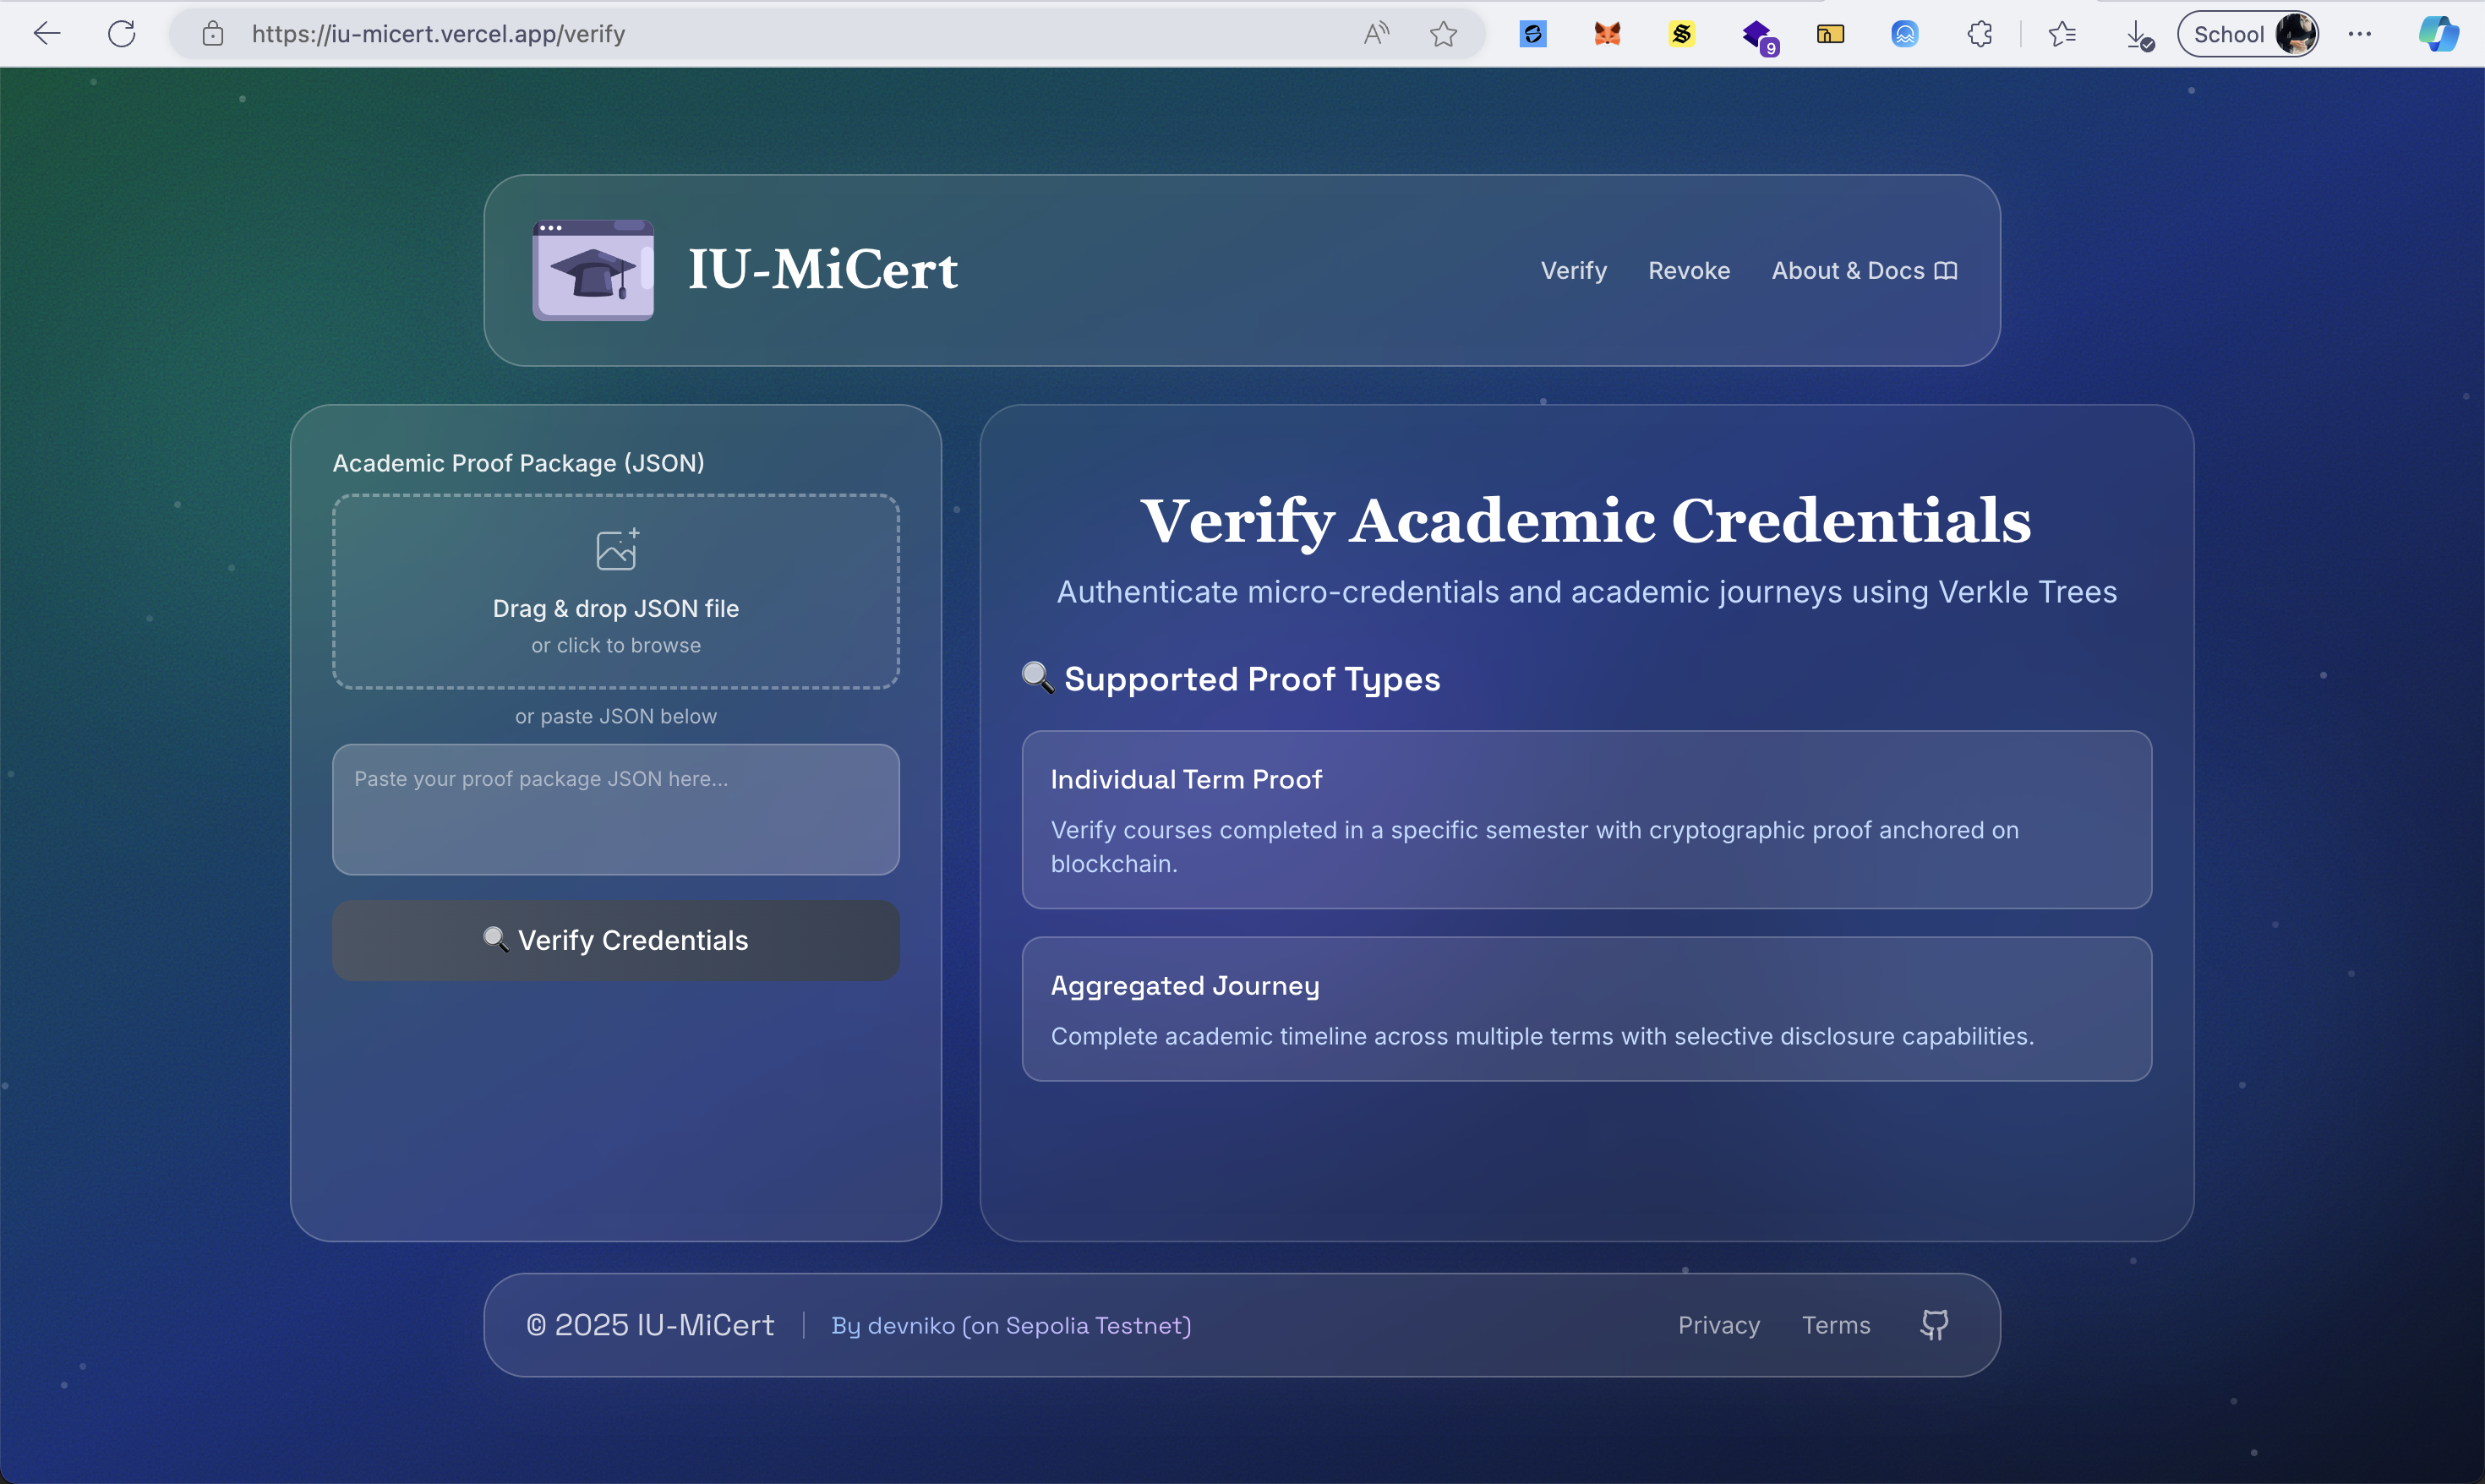
\includegraphics[width=1\textwidth]{figures/verify-ui.png}
    \caption{Main Verification Interface - Entry Point for All Receipt Types}
    \label{fig:verify-ui}
\end{figure}

The main verification interface (Figure~\ref{fig:verify-ui}) offers:
\begin{itemize}
    \item Intuitive receipt type selection
    \item Drag-and-drop upload functionality with format validation
    \item Clear workflow guidance for different verification scenarios
    \item Responsive design ensuring optimal display across all devices
\end{itemize}

\subsubsection{Single Term Verification Interface}
For focused credential verification of specific academic periods:

\begin{figure}[htbp]
    \centering
    \includegraphics[width=1\textwidth]{figures/term-verify.png}
    \caption{Single Term Verification Interface}
    \label{fig:term-verify}
\end{figure}

The single term interface (Figure~\ref{fig:term-verify}) provides:
\begin{itemize}
    \item Streamlined workflow for individual term verification
    \item Detailed credential display with comprehensive metadata
    \item Real-time verification progress indicators
\end{itemize}

\subsubsection{Academic Journey Verification Interface}
For comprehensive multi-term credential verification:

\begin{figure}[htbp]
    \centering
    \includegraphics[width=1\textwidth]{figures/journey-verify.png}
    \caption{Academic Journey Verification Interface}
    \label{fig:journey-verify}
\end{figure}

The journey verification interface (Figure~\ref{fig:journey-verify}) features:
\begin{itemize}
    \item Multi-term credential organization and display
    \item Timeline visualization for academic progression
    \item Batch verification capabilities with individual term status
    \item Comprehensive academic history presentation
\end{itemize}

\subsubsection{Academic Journey Lookup}
For advanced journey receipt management with lookup capabilities:

\begin{figure}[htbp]
    \centering
    \includegraphics[width=1\textwidth]{figures/journey-lookup-verify.png}
    \caption{Journey Lookup}
    \label{fig:journey-lookup-verify}
\end{figure}

The journey lookup interface (Figure~\ref{fig:journey-lookup-verify}) delivers:
\begin{itemize}
    \item Quick access to single terms that comprise the journey
\end{itemize}

\subsubsection{Cross-Interface Design Consistency}
All verification interfaces maintain design consistency through:
\begin{itemize}
    \item Unified color scheme and typography across all components
    \item Consistent navigation patterns and user interaction models
    \item Standardized error handling and user feedback mechanisms
    \item Responsive design principles ensuring optimal functionality across desktop, tablet, and mobile devices
\end{itemize}

\subsubsection{Accessibility and Usability Features}
The interface implementation prioritizes accessibility:
\begin{itemize}
    \item WCAG 2.1 compliance for screen reader compatibility
    \item Intuitive user flows with clear progress indicators and helpful guidance text
\end{itemize}

\section{CLI Tools Implementation Status}
\label{sec:cli_implementation}

The CLI tools component represents the next phase of development, building upon existing Verkle tree implementation experience to create comprehensive credential management utilities.

\subsection{Current Development State}
\label{subsec:cli_current_state}

While the CLI tools are not yet fully implemented, the development foundation is well-established based on previous thesis work on single diploma issuance using Verkle tree construction. The existing codebase provides:

\begin{itemize}
    \item Proven Verkle tree construction algorithms
    \item Cryptographic proof generation mechanisms
    \item Secure key management utilities
    \item Blockchain interaction capabilities
\end{itemize}

\subsection{Planned CLI Architecture}
\label{subsec:cli_architecture}

The CLI tools will be implemented in Go, leveraging the \texttt{ethereum/go-verkle} library for cryptographic operations. The planned architecture includes:

\subsubsection{Core Commands}
\begin{itemize}
    \item \texttt{micert init}: Initialize new credential repository
    \item \texttt{micert add-term}: Add new academic term with credentials
    \item \texttt{micert generate-receipt}: Create journey receipts with selective disclosure
    \item \texttt{micert verify-local}: Local verification without blockchain interaction
    \item \texttt{micert publish-roots}: Publish term root commitments to blockchain
\end{itemize}

\subsubsection{Data Format Adaptation}
The CLI implementation will adapt the existing single diploma format to support:
\begin{itemize}
    \item Multi-term credential structures
    \item Hierarchical academic progression
    \item Selective disclosure metadata
    \item Temporal consistency validation
\end{itemize}

\subsection{Implementation Roadmap}
\label{subsec:cli_roadmap}

The CLI development follows a phased approach:

\begin{enumerate}
    \item \textbf{Phase 1}: Adapt existing Verkle tree implementation for multi-term support
    \item \textbf{Phase 2}: Implement journey receipt generation with selective disclosure
    \item \textbf{Phase 3}: Integrate blockchain publishing capabilities
    \item \textbf{Phase 4}: Add comprehensive testing and validation utilities
\end{enumerate}

The implementation leverages proven cryptographic libraries and follows established security practices from the previous diploma issuance system.

% TODO: Add CLI command structure diagram
% \begin{figure}[htbp]
%     \centering
%     \includegraphics[width=0.8\textwidth]{figures/cli_structure.png}
%     \caption{Planned CLI Command Structure}
%     \label{fig:cli_structure}
% \end{figure}

\section{Blockchain Implementation Approach}
\label{sec:blockchain_implementation}

The blockchain component implementation strategy leverages existing verification capabilities while exploring enhanced system architectures for improved efficiency and functionality.

\subsection{Current Blockchain Integration Status}
\label{subsec:blockchain_status}

The blockchain integration is in the planning and design phase, with implementation strategies informed by previous thesis work on on-chain credential verification. The current understanding includes:

\begin{itemize}
    \item Proven feasibility of on-chain Verkle proof verification
    \item Smart contract capabilities for credential validation
    \item Gas optimization strategies for batch operations
    \item Integration patterns with frontend applications
\end{itemize}

\subsection{Implementation Strategies}
\label{subsec:blockchain_strategies}

Two primary approaches are being considered for blockchain implementation:

\subsubsection{Direct Verification Approach}
The direct approach involves:
\begin{itemize}
    \item Individual term verification through separate smart contract calls
    \item Straightforward implementation using existing proof verification functions
    \item Higher gas costs but simpler smart contract logic
    \item Direct compatibility with current frontend verification workflows
\end{itemize}

This approach provides immediate functionality by adapting existing single-term verification to handle multiple terms sequentially.

\subsubsection{Enhanced Batch Verification}
The enhanced approach focuses on:
\begin{itemize}
    \item Batch verification of multiple terms in single transactions
    \item Optimized gas usage through aggregated proof validation
    \item Complex smart contract logic for journey receipt validation
    \item Advanced cryptographic operations for efficient verification
\end{itemize}

This approach requires more sophisticated implementation but offers superior performance and cost-effectiveness for large-scale deployments.

\subsection{Smart Contract Architecture}
\label{subsec:smart_contract_architecture}

The planned smart contract architecture builds upon the pseudocode outlined in Chapter \ref{ch:methodology} (Methodology), extending functionality to support:

\subsubsection{Enhanced Storage Management}
\begin{itemize}
    \item Hierarchical term organization by academic periods
    \item Efficient root commitment storage with metadata
    \item Revocation management with granular control
    \item Access control for authorized credential issuers
\end{itemize}

\subsubsection{Advanced Verification Functions}
\begin{itemize}
    \item Batch verification capabilities for journey receipts
    \item Temporal consistency validation across multiple terms
    \item Academic progression rule enforcement
    \item Selective disclosure support with privacy preservation
\end{itemize}

\subsection{Development Priorities}
\label{subsec:blockchain_priorities}

The blockchain implementation prioritizes:

\begin{enumerate}
    \item \textbf{Security}: Comprehensive cryptographic validation and access control
    \item \textbf{Efficiency}: Gas-optimized operations for cost-effective verification
    \item \textbf{Compatibility}: Seamless integration with existing frontend and CLI components
    \item \textbf{Scalability}: Architecture supporting high-volume credential verification
\end{enumerate}

The implementation will begin with the direct verification approach to establish baseline functionality, followed by enhancement to batch verification for improved performance.

% TODO: Add blockchain interaction flow diagram
% \begin{figure}[htbp]
%     \centering
%     \includegraphics[width=0.8\textwidth]{figures/blockchain_flow.png}
%     \caption{Blockchain Verification Workflow}
%     \label{fig:blockchain_flow}
% \end{figure}

\section{Integration and Testing Strategy}
\label{sec:integration_testing}

The implementation strategy emphasizes thorough integration testing and validation across all system components to ensure reliable operation and security.

\subsection{Component Integration}
\label{subsec:component_integration}

The integration approach follows a systematic methodology:

\begin{enumerate}
    \item \textbf{Frontend-CLI Integration}: Ensuring seamless data flow between web interface and command-line tools
    \item \textbf{CLI-Blockchain Integration}: Validating smart contract interactions and transaction handling
    \item \textbf{End-to-End Workflows}: Complete credential lifecycle testing from issuance to verification
    \item \textbf{Cross-Component Validation}: Ensuring data consistency and format compatibility
\end{enumerate}

\subsection{Testing Framework}
\label{subsec:testing_framework}

The testing strategy encompasses:

\subsubsection{Unit Testing}
\begin{itemize}
    \item Individual component functionality validation
    \item Cryptographic operation correctness verification
    \item Data format and serialization testing
    \item Error handling and edge case coverage
\end{itemize}

\subsubsection{Integration Testing}
\begin{itemize}
    \item Cross-component communication validation
    \item Blockchain transaction testing on Sepolia testnet
    \item Performance benchmarking for large credential sets
    \item Security audit of cryptographic implementations
\end{itemize}

\subsubsection{User Acceptance Testing}
\begin{itemize}
    \item Realistic workflow simulation with generated test data
    \item User interface usability evaluation
    \item Performance testing under various load conditions
    \item Compatibility testing across different browser environments
\end{itemize}

\section{Current Limitations and Future Enhancements}
\label{sec:limitations_enhancements}

The current implementation state presents several limitations that will be addressed in future development phases:

\subsection{Current Limitations}
\label{subsec:current_limitations}

\begin{itemize}
    \item \textbf{CLI Tools}: Not yet implemented, limiting end-to-end credential management capabilities
    \item \textbf{Blockchain Integration}: Pending implementation of smart contract verification system
    \item \textbf{Scalability Testing}: Limited validation with large-scale credential datasets
    \item \textbf{Production Deployment}: Current implementation focused on development and testing environments
\end{itemize}

\subsection{Planned Enhancements}
\label{subsec:planned_enhancements}

Future development will address current limitations through:

\begin{itemize}
    \item \textbf{Complete CLI Implementation}: Full command-line utility suite for credential management
    \item \textbf{Advanced Blockchain Features}: Enhanced smart contract capabilities with batch verification
    \item \textbf{Performance Optimization}: Improved efficiency for large-scale credential processing
    \item \textbf{Security Auditing}: Comprehensive security analysis and vulnerability assessment
    \item \textbf{Production Readiness}: Deployment optimization and monitoring capabilities
\end{itemize}

\section{Chapter Summary}
\label{sec:implementation_summary}

This chapter has presented the current implementation state of the IU-MiCert system, highlighting the completed frontend components, planned CLI tools development, and blockchain integration strategy. The implementation demonstrates significant progress in creating a comprehensive decentralized credential management system with advanced privacy features.

The frontend implementation provides a robust foundation for credential verification and receipt management, supporting multiple verification types and selective disclosure capabilities. The planned CLI tools development builds upon proven Verkle tree implementation experience, while the blockchain integration strategy balances immediate functionality with long-term performance optimization.

The systematic approach to implementation ensures that each component contributes effectively to the overall system architecture while maintaining security, efficiency, and user experience standards. The integration and testing strategy provides confidence in system reliability and prepares for future enhancements and production deployment.

The current progress establishes a solid foundation for the complete IU-MiCert system implementation, with clear development paths for the remaining components and a comprehensive understanding of the technical challenges and solutions involved in decentralized credential management.
\chapter{RESULT}
\label{ch:result}
[To be completed after system implementation and testing]
\chapter{DISCUSSION}
\label{ch:discussion}
[To be completed after results analysis]
\chapter{CONCLUSION}
\label{ch:conclusion}
[To be completed after full thesis work]

% Bibliography
\bibliographystyle{ieeetr}
\bibliography{reference}

\end{document}